\hypertarget{introduction}{%
\section{Introduction}\label{introduction}}

This report describes the creation of the new Industry Exchange Network
website showcasing UCL Computer Science student's projects and marketing
the organisation to attract new industry partners.

\hypertarget{the-client}{%
\subsection{The Client}\label{the-client}}

The IXN project was appointed by Dr Yun Fu, a Teaching Fellow, App
Project Manager and Student Internship Manager at University College
London (UCL). An important part of Dr Fu's profession is to connect
students to the industry, therefore, having a website to showcase the
work done by the Computer Science department to the industry is
significant. Consequently, the Industry Exchange Network (IXN) website
was commissioned with the intent to bridge the gap between students and
industry

\hypertarget{the-project}{%
\subsection{The Project}\label{the-project}}

The Industry Exchange Network website allows UCL Computer Science
students to get involved with term-based client projects \cite{g1}. The
website showcases a variety of student projects, ranging from 1st Year
Students to the more advanced MSc Data Science endeavours. The clients
are entrepreneurs, charities, healthcare companies, researchers, SMEs,
the government and large enterprises. The IXN website is a platform to
allow individuals in the industry to get in touch with the members of
the IXN team. The main objective of the website, therefore, is to market
IXN to professionals; showcasing the abilities of UCL Computer Science
students.

\hypertarget{website-overview}{%
\subsection{Website Overview}\label{website-overview}}

\begin{figure}[H]
      \centering
      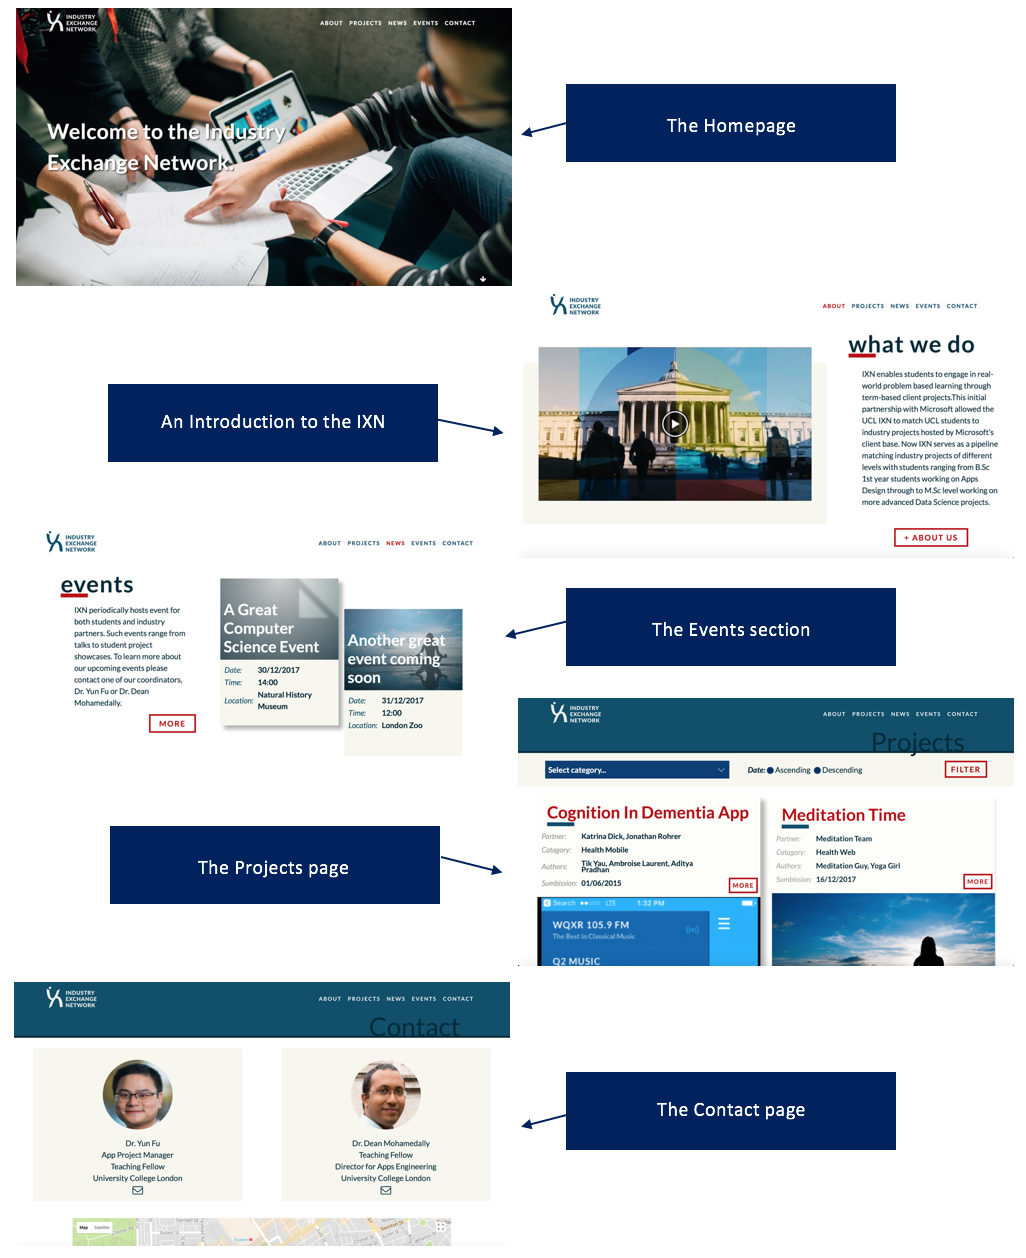
\includegraphics[trim = 0 0 0 0, clip, width=0.98\textwidth]{ph13.png}
 \end{figure}

\hypertarget{project-management}{%
\section{Project Management}\label{project-management}}

\hypertarget{the-team}{%
\subsection{The Team}\label{the-team}}

\hypertarget{alexander-charles-team-leader}{%
\subsubsection{Alexander Charles (Team
Leader)}\label{alexander-charles-team-leader}}

Alexander obtained a Bachelor of Engineering in Engineering Design
specialising in Aerospace. He has worked firms ranging from Babcock
International in Marine and Defence, a centre of manufacturing research
excellence named the Manufacturing Technology Centre and has lately
transitioned into Strategy consulting working on advising
Telecommunications CEO's on the use of blockchain technology while at
Redshift Strategy. In his spare time, Alexander has practised web
development, building WordPress website for an array of small clients.

\textbf{Roles:} - Project Management - Front End-Development and
Optimisation - Back-end Development and Deployment - UI Design -
Prototyping - Report Writing

\hypertarget{giovanni-tenderini}{%
\subsubsection{Giovanni Tenderini}\label{giovanni-tenderini}}

Giovanni obtained a Bachelor of Science in Economics and Finance at the
University of Exeter. His work experience includes a Summer Internship
in the Investment Banking division of a Family Office in Milan named CFO
and another internship at Generali Italia insurance sales division. His
overall knowledge in programming skills is basic. However, he is an
expert in statistical analysis and some related programs.

\textbf{Roles:} - Testing - Sketching and Design - Prototyping - Final
and Weekly report writing - Video making - Minimal Front-End
implementation

\hypertarget{phoebe-staab}{%
\subsubsection{Phoebe Staab}\label{phoebe-staab}}

A graduate of the BSc Chemistry Programme at University College Dublin,
Phoebe had little to no real programming experience before attending
UCL. She had done a couple of online courses in Java and Python and did
some novice-level statistics programming in R during her undergraduate
degree.

\textbf{Roles:} - Prototyping - Front End-Development - Report Writing -
Content creator - Research - Minimal Back-end development

\hypertarget{team-coordination}{%
\subsection{Team Coordination}\label{team-coordination}}

In team projects, good organisation is fundamental to effective
collaboration. Productivity tools and workflow management has been key
to the team working efficiently. The key technologies used by the IXN
team included: - \textbf{Slack:} allowing team members to communicate.
Chosen due to its ability to share files, track conversations via thread
and create alerts - \textbf{Trello:} used as a dashboard to distinguish
between work to be done, in progress or completed - \textbf{OneDrive:}
was used as a cloud sharing tool. Usually, for confidentiality reasons,
clients require their repository to be private.\\
- \textbf{GitHub:} used to share code between developers, provide
version control, manage conflicts and deploy the site to the live
server. A private repository provided by UCL was used to keep any work
out of the public domain

\hypertarget{scheduling}{%
\subsection{Scheduling}\label{scheduling}}

Work packages were allocated according to each team members' strengths
and weaknesses. Jobs were distributed to optimise team members time
while allowing all individuals to learn. A Gantt chart was used to map
out the timeline of the project to keep tasks on track and manage
deadlines. Figure \ref{gantt}, shows a slimmed down version of the Gantt
chart used.

\begin{figure}[H]
      \centering
      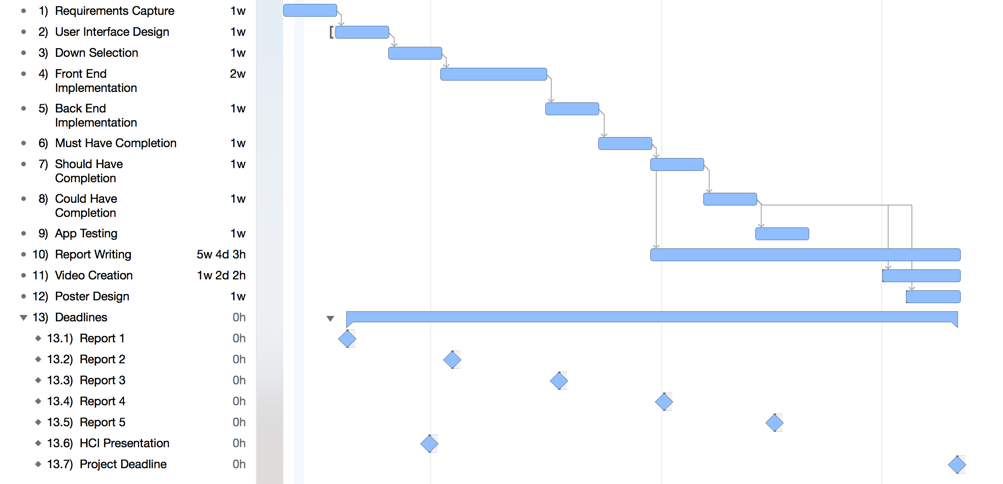
\includegraphics[trim = 0 0 0 0, clip, width=0.98\textwidth]{Picture1.png}
      \caption{Gantt chart where "w" stands for weeks dedicated to the development of each task}
\label{gantt}
 \end{figure}

\hypertarget{requirements}{%
\section{Requirements}\label{requirements}}

\hypertarget{client-requirements}{%
\subsection{Client Requirements}\label{client-requirements}}

The requirements of the website were highlighted in the first meeting
with Dr Yun Fu. The existing website for the IXN network was shown to
the group and presented design, content and responsiveness issues. In
fact, the aim of the Industry Exchange Network website is to be guide
and convince industry leaders to join by contacting the administrators,
such a problematic website was not suitable to represent the Computer
Science department at UCL. Therefore, new website had to be a high
quality exemplification of what the department is able to do and the
following features were required by the client:

\begin{itemize}
\tightlist
\item
  High quality and professional design
\item
  Fully responsive website
\item
  Content management system to allow the Administrator to update the
  website without touching code
\item
  Separate sections for Events, News and Featured Projects.
\item
  A navigation bar always present at the top of the website
\end{itemize}

\hypertarget{design-process}{%
\section{Design Process}\label{design-process}}

In order to be able to complete the project to both a high standard an
within a timely manner, a design process was following both process and
agile design methods to reach the projects objectives. The project was
spilt into three phases: \emph{definition, design} and
\emph{development}. Figure \ref{designprocess}, shows an overview of the
projects workflows and a breakdown of the key steps of each phase.

\begin{figure}[H]
\centering
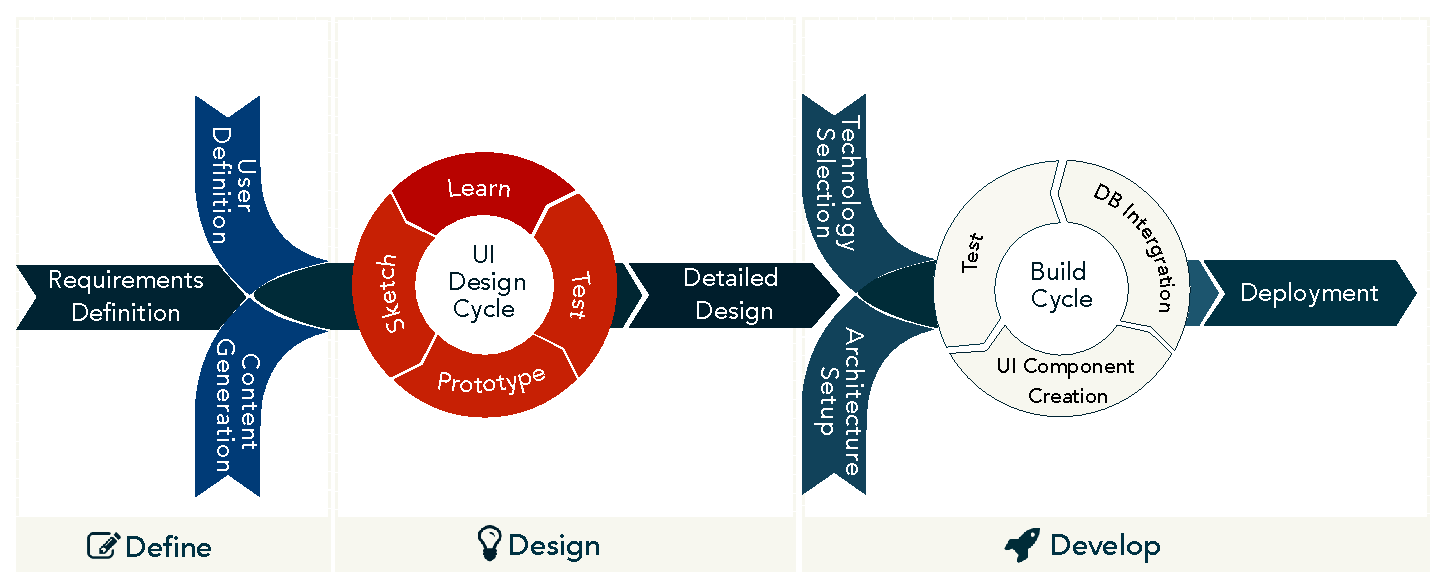
\includegraphics[trim = 0 0 0 0, clip, width=0.98\textwidth]{DesignProcess.eps}
\caption{Diagram illustrating the design process progressing the from the initial briefing to implementation}
\label{designprocess}
\end{figure}

\hypertarget{definition-phase}{%
\subsection{Definition Phase:}\label{definition-phase}}

This phase focused on collecting requirements and defining the
objectives of the project. In order to capture all the information
correctly, several meetings were held with the client these meetings
meetings were used to capture the main features of the site, creating
and organising the content that would be displayed. User research was
then embarked, refining the objectives and content of the site. These
stages all worked towards providing all the prior research required to
begin designing, prototyping and envisioning how the website would
function.

\hypertarget{design-phase}{%
\subsection{Design Phase:}\label{design-phase}}

The design phase applied human computer interaction (HCI) principles in
an agile to approach, to mock up variety of different solutions and
refine the solutions quickly. By following of the process of creating
sketches of different components of the website, whittling these
sketches down to wireframes and prototypes. Solutions could be quickly
tested by the designers, client and user groups providing feedback to
take back and learn upon, improving the overall design of the website
until a rough solution was generated which met both the design
objectives and the met HCI objectives. Spending time before writing any
code was key to making sure the solution was user friendly and visual
meeting one of the key objectives of the project. After rough solution
was created through user interface (UI) design cycle, this was then
padded out and refined creating a static draft of the design which could
be directly copied in the development phase. A large amount of time
could be saved in the development phase of the project by having a
finalised design template to work of which included the typography,
components and the page layouts of the site.

\hypertarget{development-phase}{%
\subsection{Development Phase:}\label{development-phase}}

Development was the final phase of the project. A complete understanding
of how the final product will look and function, based on the research
conducted in the definition phase and the detailed design template in
the design phase meant that all the technology required to required to
implement the solution can be selected. A local development environment
shared amongst all the developers enabled the use of an agile build
cycle, using git to mediate between the different versions. The build
cycle consisted of a developer taking a UI component from the template
and creating the design in code. This would then be connected to the PHP
database using word-press and the tested. Any bugs in either the design
or functionality could then be ironed out through iteration through the
cycle eventually integrating all the components together into the final
site. Once the entire design template was implemented the project could
then be deployed onto the web.

\newpage

\hypertarget{user-research}{%
\section{User Research}\label{user-research}}

\hypertarget{round-one-user-feedback}{%
\subsection{Round One User Feedback}\label{round-one-user-feedback}}

A first round of user surveys was taken based on sketches in order to
assess necessary content. The results were used to inform a MoSCoW,
storyboards, and subsequent sketches. Evaluation is concerned with
gathering the usability of a design or a product by a specified group of
users within a specified environment or work context. The results of the
survey are outlined below:

\begin{figure}[H]
      \centering
      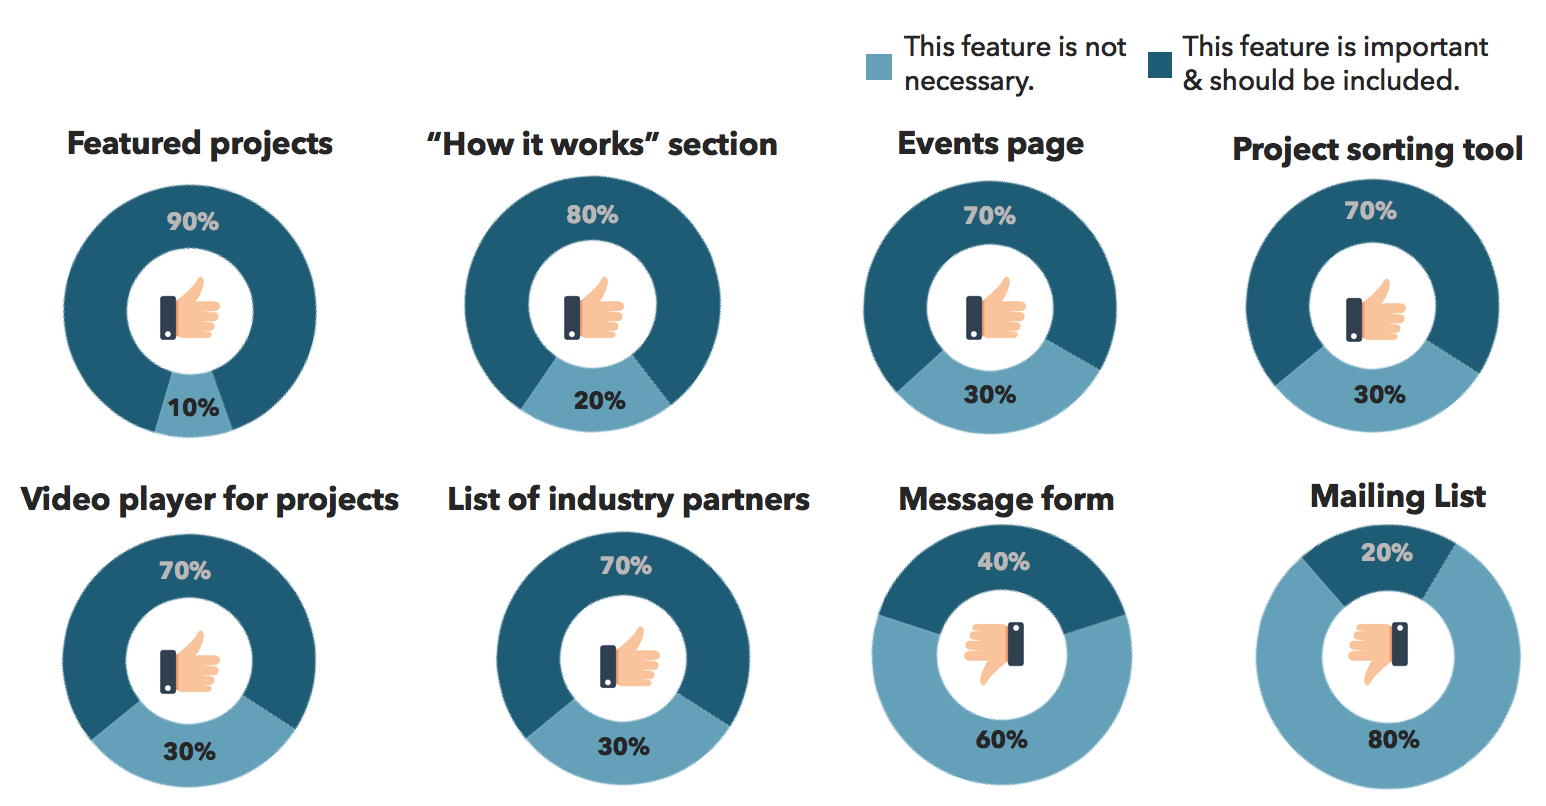
\includegraphics[trim = 0 0 0 0, clip, width=0.7\textwidth]{ph3.png}
      \caption{IXN network round one User Feedback result summary}
 \end{figure}

As it can be seen, the features which are given more importance are the
ones related to the showcasing of projects, enforcing the fact that the
quality of the design is of fundamental importance for IXN. Indeed,
industry individuals who are thinking of relying on IXN for their
ventures would feel comforted by seeing past projects displayed in a
skilled and professional way.

\hypertarget{related-readings}{%
\subsection{Related Readings}\label{related-readings}}

Related readings were highly important due to the red tape imposed on
research by regulations at UCL. External sources were used to understand
the type of audience the website would appeal to and what level of
digital ability the users typical would have. The image below shows the
main findings:

\begin{figure}[H]
      \centering
      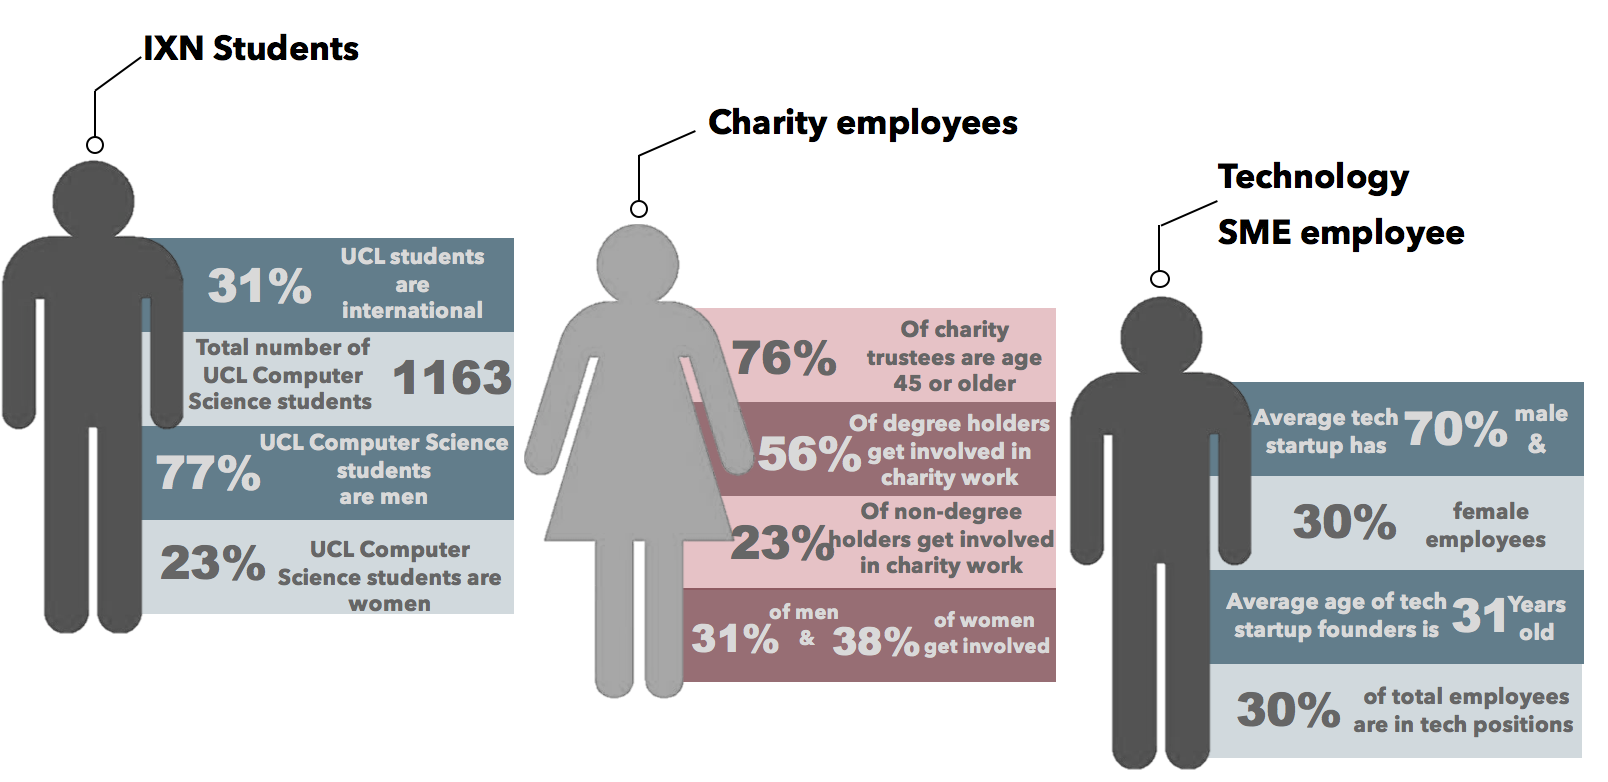
\includegraphics[trim = 0 0 0 0, clip, width=0.7\textwidth]{p21.png}
      \caption{Summarized statistics extracted from the readings explaied below}
 \end{figure}

Data providing a fuller picture of the demographics of IXN Students was
found primarily using UCL student statistics \cite{ps1}. This
information was provided on the UCL website. It was determined that the
IXN student audience is typically british and male. This evidence helped
us develop a data-driven persona. The client indicated that this is not
a target-user, but never the less, user research determined that UCL IXN
student would be an audience regardless of the website's intent, since
they would like to see their work, the work of other students, and
possible industry partners.

The client's target audience for the IXN site was potential and current
partners. Based on the assigned projects for GC02 during the current
term, the partners tend to be from technology companies and charity
institutions.

Research was done on the demographics of a typical charity volunteer/
employee in the United Kingdom using sources such as The Charity
Commission \cite{ps2} and National Council for Voluntary Organisations
\cite{ps3}. Based on worked published from these organizations, it was
determined that the typical charity employee was aged 45 or older and
usually holds a degree. A persona and use-case was developed regarding
this data. This data also indicated that the site should be streamlined
and simple without confusion on how to navigate through different pages.

In order to obtain a profile for a technology employee sources such as
the Atlantic \cite{ps4} and The Harvard business review \cite{ps5} were
utilized. The research indicated that employees at such businesses are
typically males in their early to mid thirties. This data was, again,
used to inform a persona/ use-case. It was determined that this type of
user is typically technology-proficient and that the site should reflect
the high calibre of technical capability of IXN students.

\hypertarget{limitations}{%
\subsection{Limitations}\label{limitations}}

The main limitations were imposed by the decision taken by the HCI
department which did not allow questionnaires to be shown and completed
by people outside of the computer science department. Fortunately, in
the case of the Industrial Exchange Network UCL Computer Science
students account to a high percentage of its users. To enable more in
depth research for our website having more time to dedicate to research
could have helped to broaden the number of people questioned. Having a
budget to dedicate to research could have also helped to obtain more
statistically significant results. For example, questionnaires could
have been sponsored to attract a larger public to complete them.

\hypertarget{users-and-personas}{%
\subsection{Users and personas}\label{users-and-personas}}

Based on client specification and demographics research, 5 personas were
created to gain understanding of the end user of the product. Please
refer to Figure ``X'' in the Appendix for detailed personas. The two
main user categories to focus on are: ​

• Small-Medium Tech Enterprise Owners: ​ - Digital Native Users who have
got strong tech background​ - Look for a business opportunity​ - High
expectations from design and quality of website​ - The platform has to
appear professional for them to be incentivised to join IXN​.

The main design principles which have to be considered for this specific
persona are: ​ consistency: essential for a professional looking
website​ affordance: for an intuitive interaction with the platform. ​

\begin{figure}[H]
      \centering
      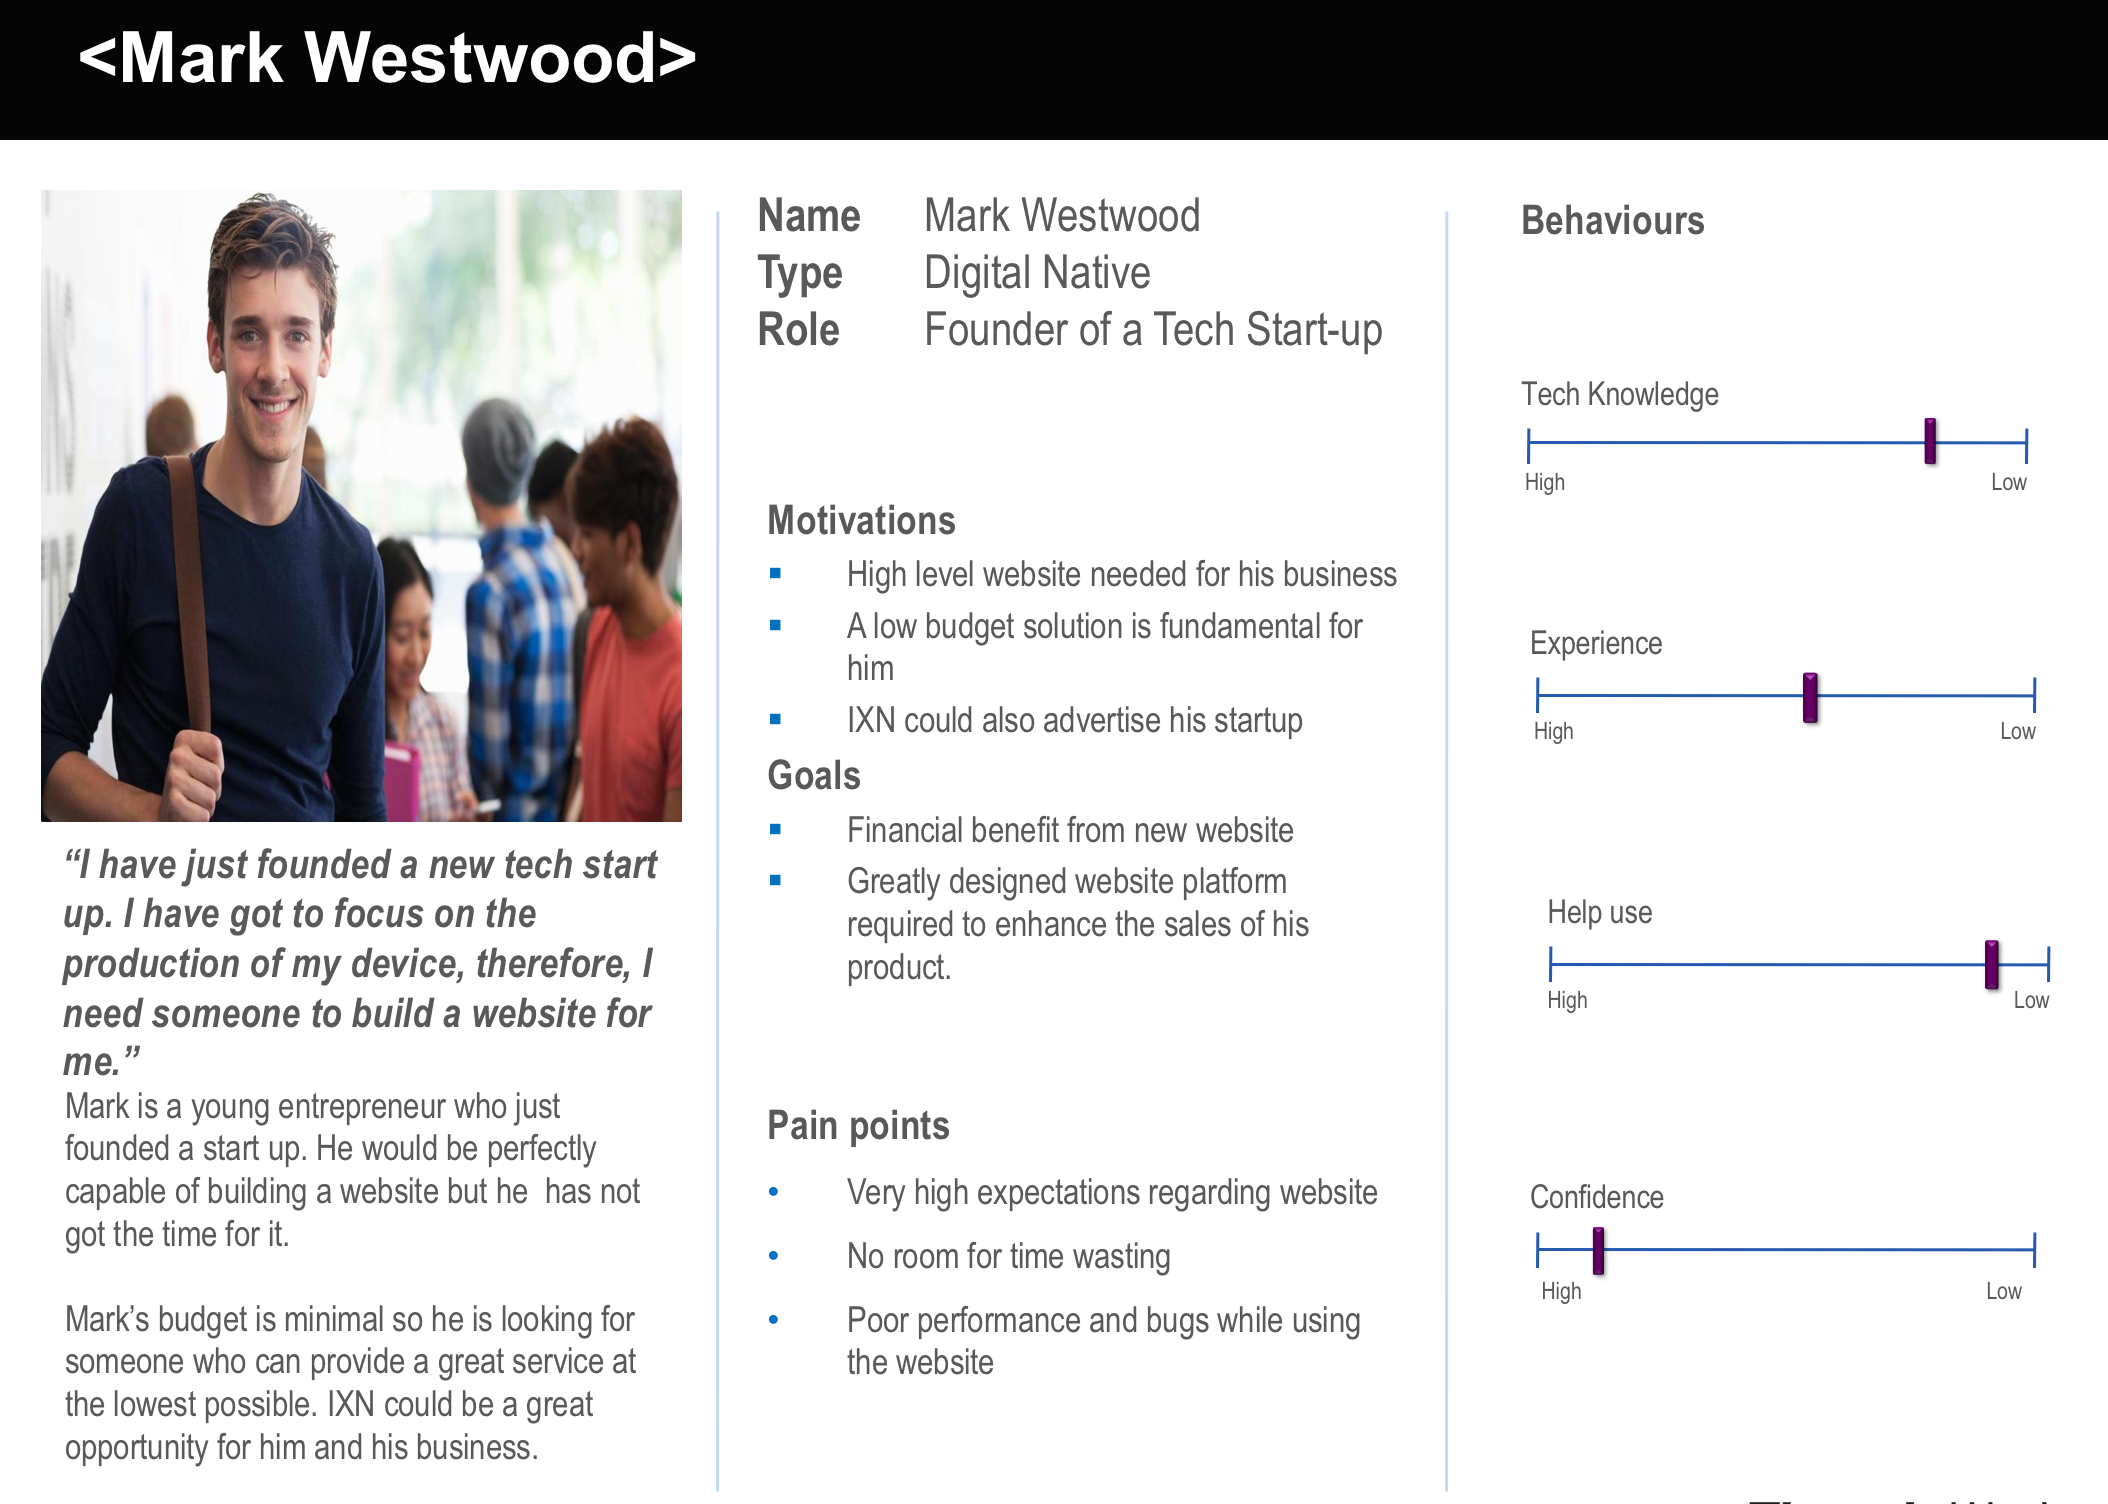
\includegraphics[trim = 0 0 0 0, clip, width=0.7\textwidth]{ph1.png}
      \caption{SME Tech Enterprise Owner}
\end{figure}

• UCL Computer Science Students: ​ - Highly trained digital users​ -
They require the projects they have worked on to be very visible​ -
Expect to be well represented by the design of the website​ - They
desire the platform to be as entertaining as possible. ​

The main design principle which has to be considered for this specific
persona is: ​ visibility: especially in relation to how the projects are
showcased. ​

\begin{figure}[H]
      \centering
      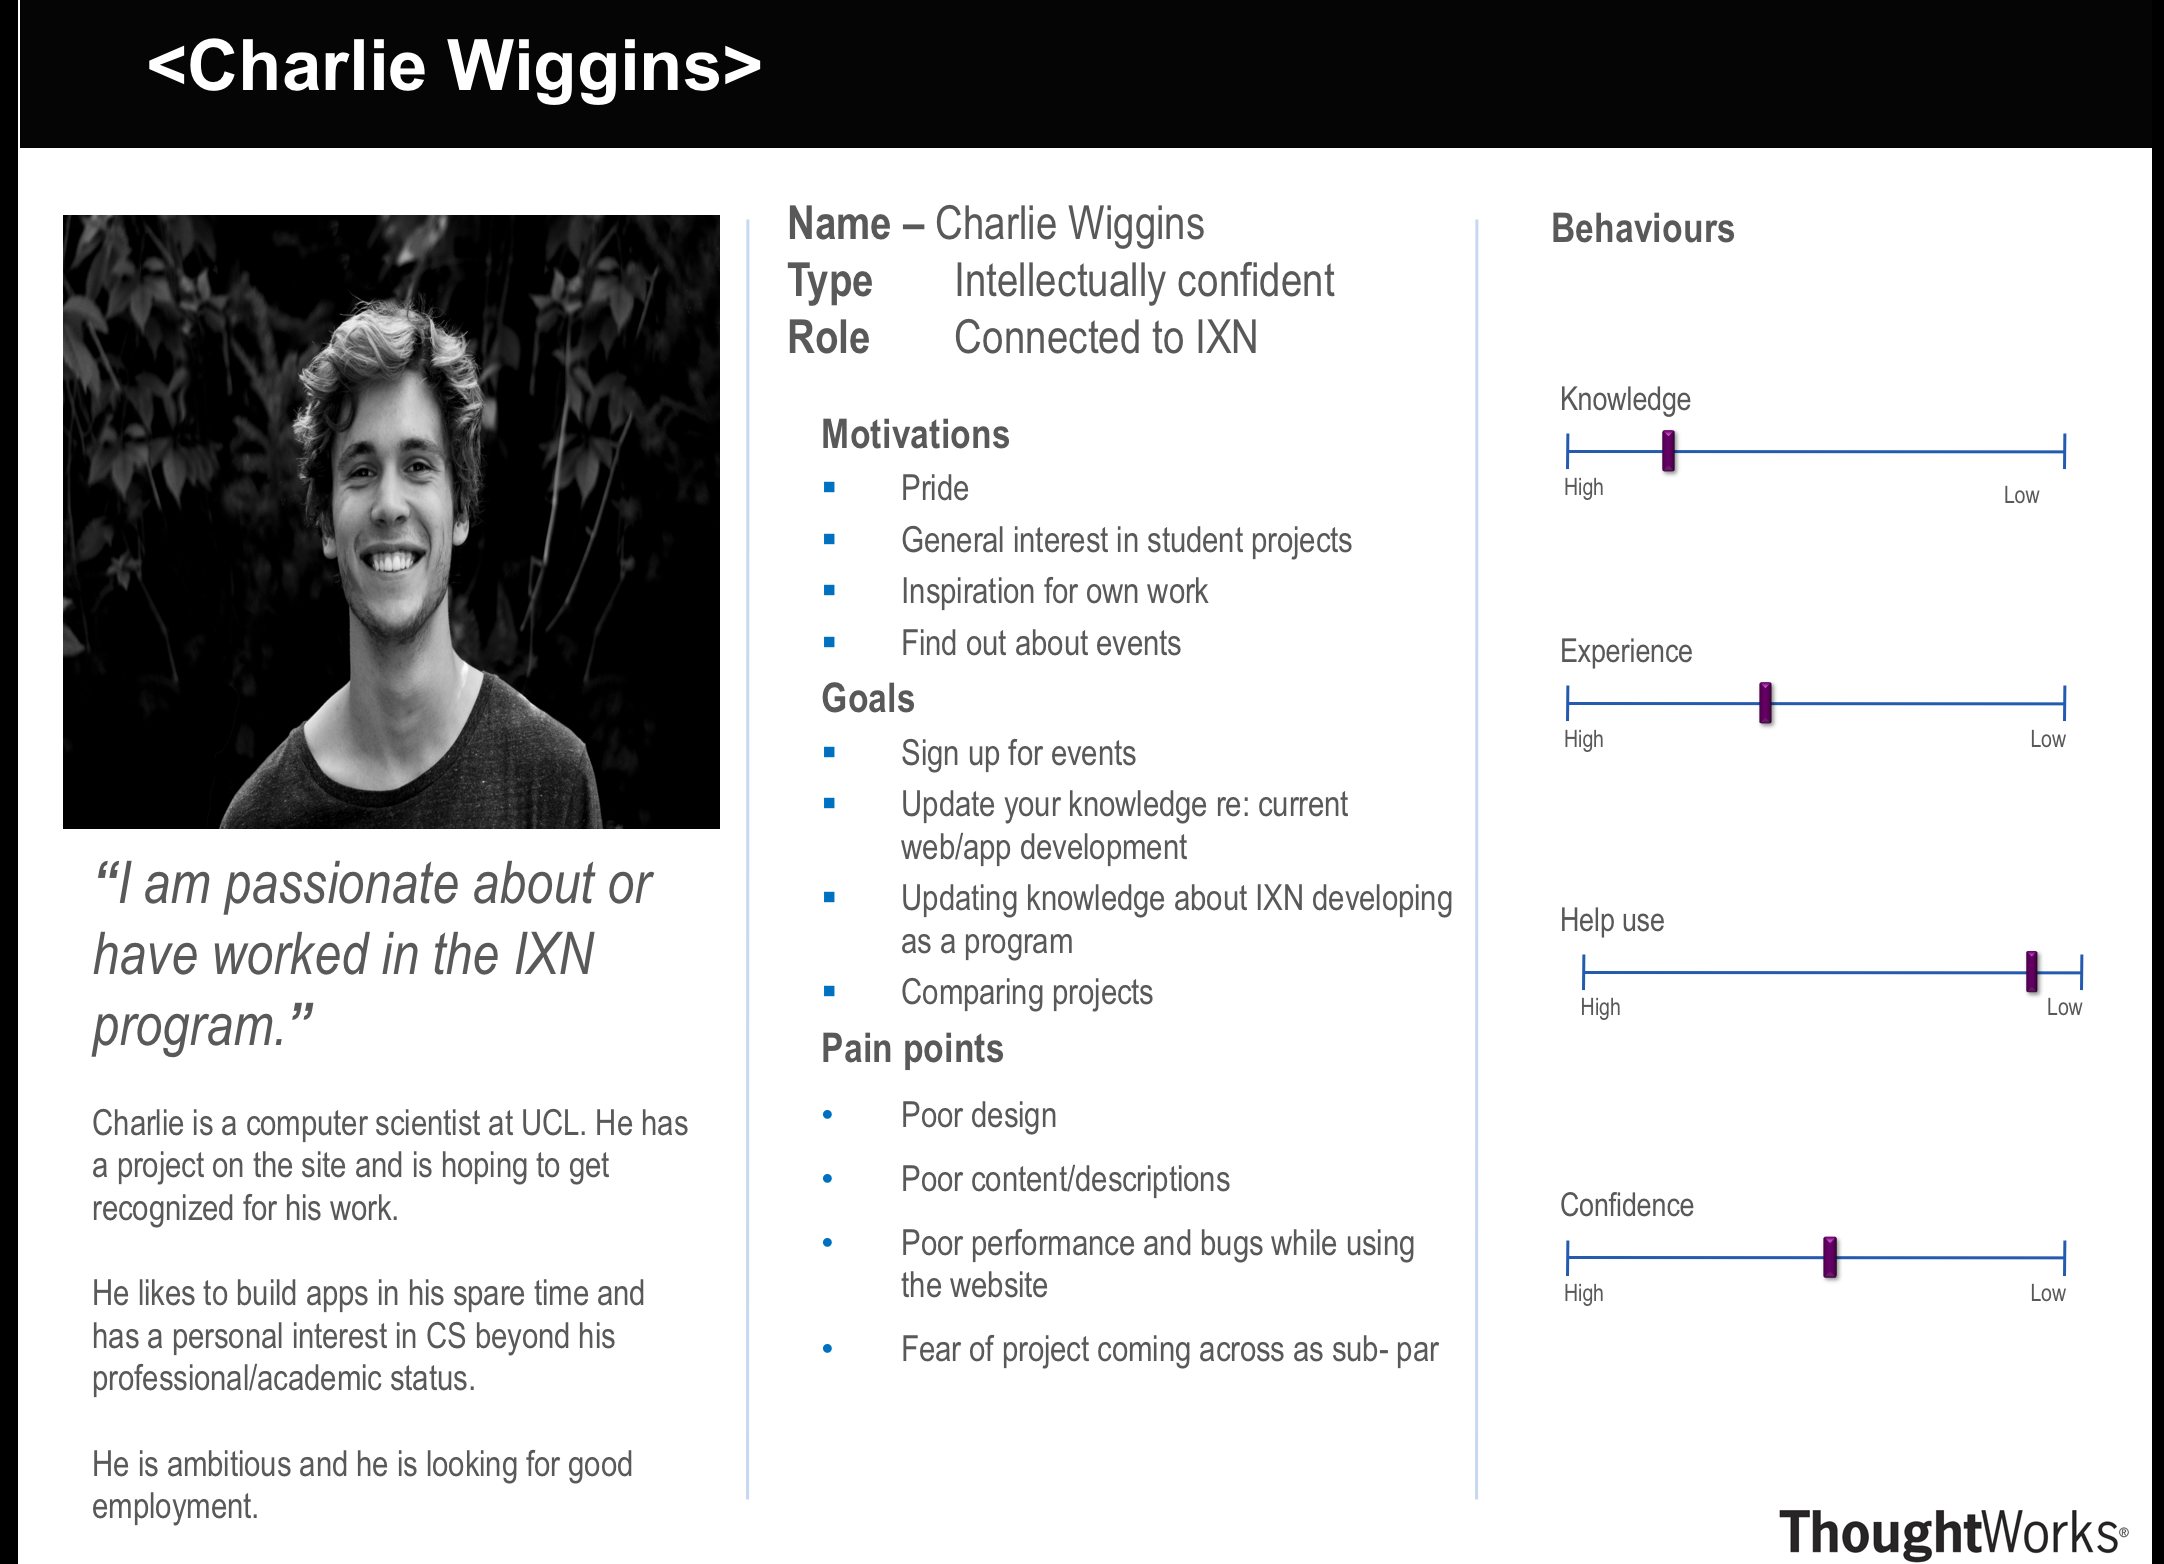
\includegraphics[trim = 0 0 0 0, clip, width=0.7\textwidth]{persona1.png}
      \caption{UCL Computer Science Student}
\end{figure}

Use Cases

Use cases are constructed to represent the standard user navigation and
interaction with the platform needed to accomplish a given task
\cite{g3}. These are useful to shape the development and design of the
website, facilitating the interaction between the website and its users.
In the case of the IXN website the role of the administrator has also
been taken into account.

\begin{figure}[H]
      \centering
      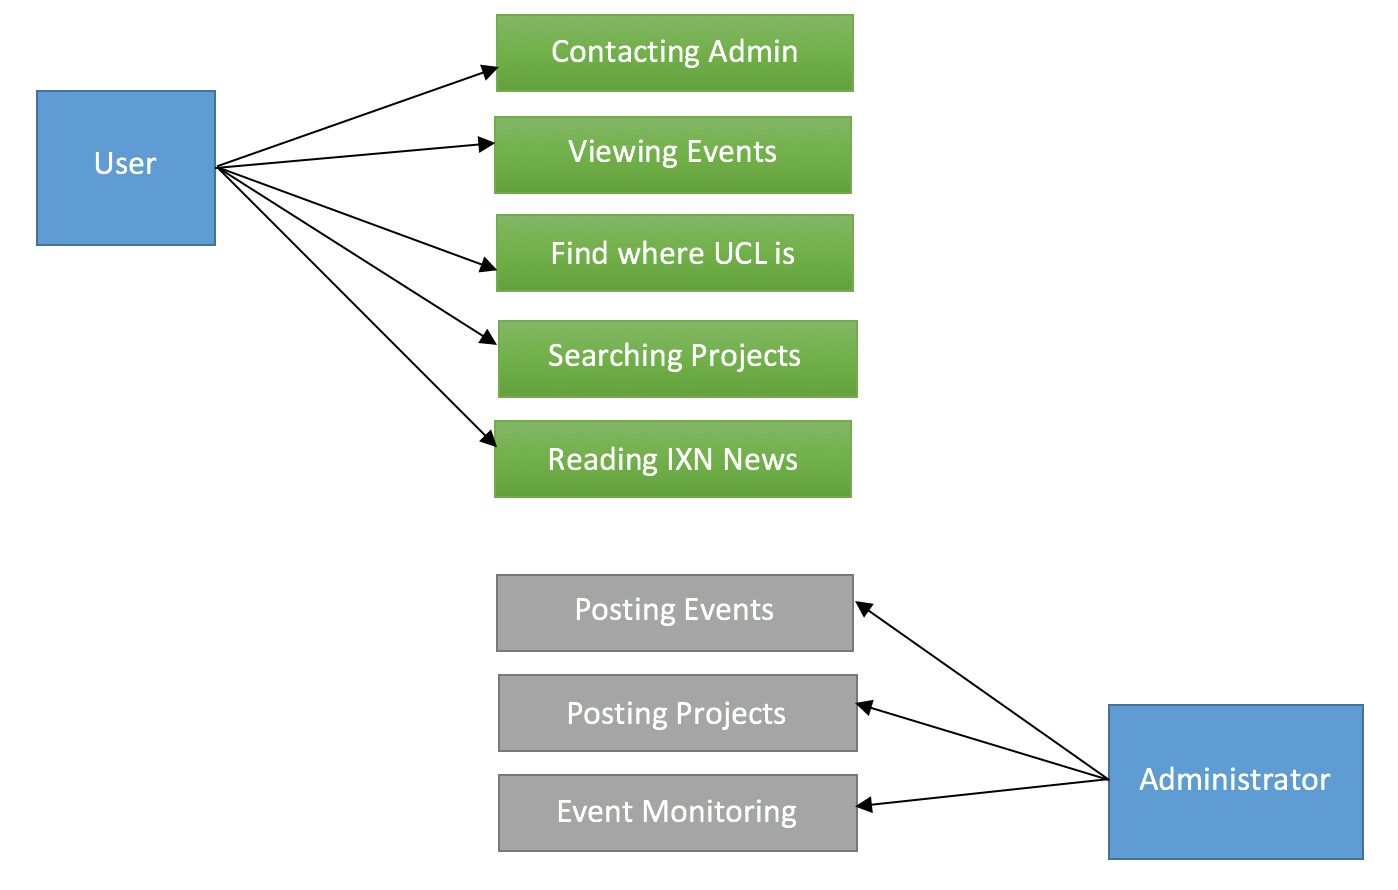
\includegraphics[trim = 0 0 0 0, clip, width=0.7\textwidth]{ph9.png}
      \caption{Use case graph}
\end{figure}

An outline of the use cases can be found below. This is essentially a
list of the actions realated to the Must and Should sections of the
MoSCoW. To avoid repetition, the main routes (in bold) have been
outlined in detail.

\begin{figure}[H]
      \centering
      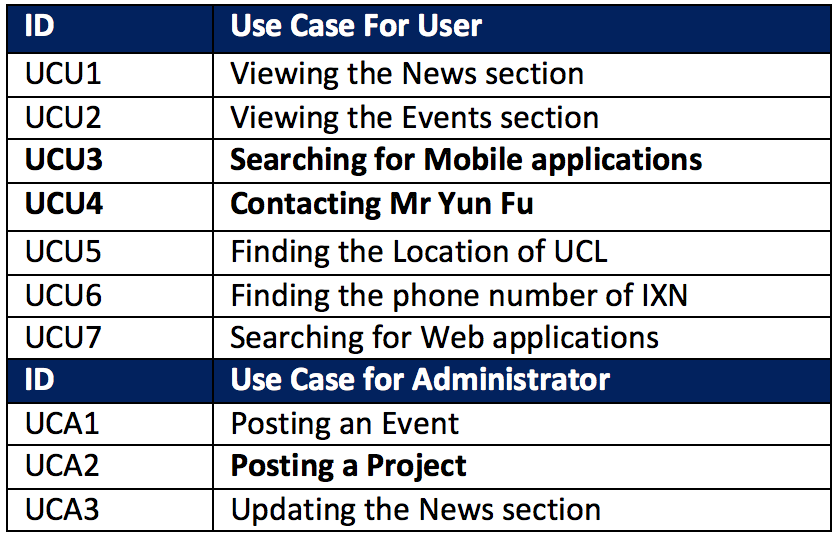
\includegraphics[trim = 0 0 0 0, clip, width=0.7\textwidth]{ph10.png}
      \caption{Use case list}
 \end{figure}

\begin{figure}[H]
      \centering
      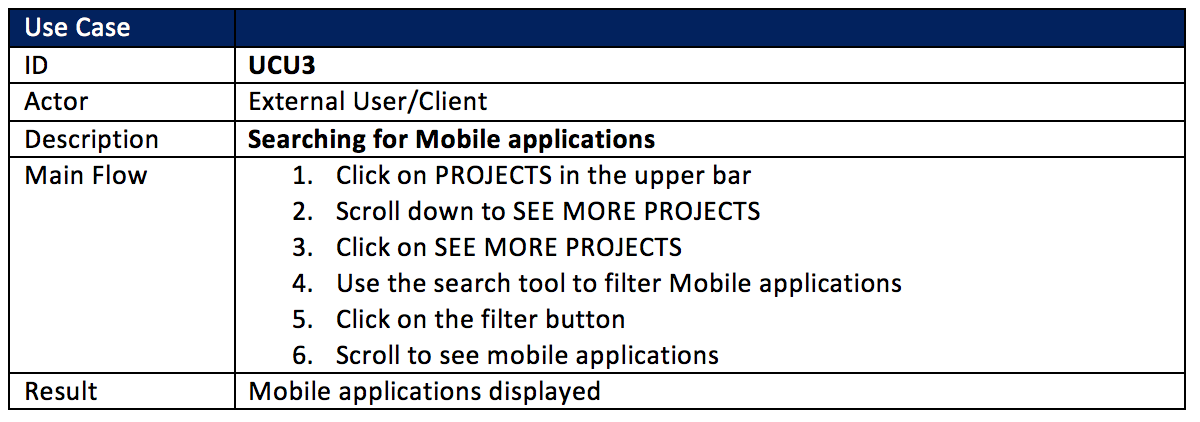
\includegraphics[trim = 0 0 0 0, clip, width=0.7\textwidth]{ph12.png}
      \caption{Detailed UCU3}
 \end{figure}

\begin{figure}[H]
      \centering
      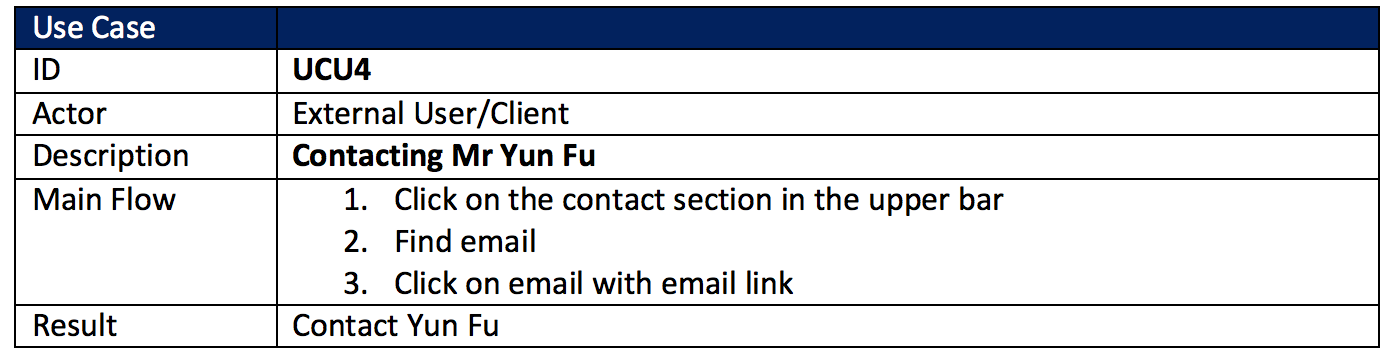
\includegraphics[trim = 0 0 0 0, clip, width=0.7\textwidth]{ph11.png}
      \caption{Detailed UCU4}
 \end{figure}

\hypertarget{mosccow}{%
\subsection{MoScCoW}\label{mosccow}}

To distinguish between Must Have requirements, Should and Could Haves
the team used a MoSCoW analysis framework \cite{g4}. The tool was
constructed by combining statistics extracted form a questionnaire posed
to UCL students, Client Requirements, Personas and Use Cases. A well
developed MoSCoW facilitates the implementation and design of a project
by streamlining the creation and implementation processes. Below in
figure ``X'' the MoSCoW of the IXN project is displayed:

\begin{figure}[H]
      \centering
      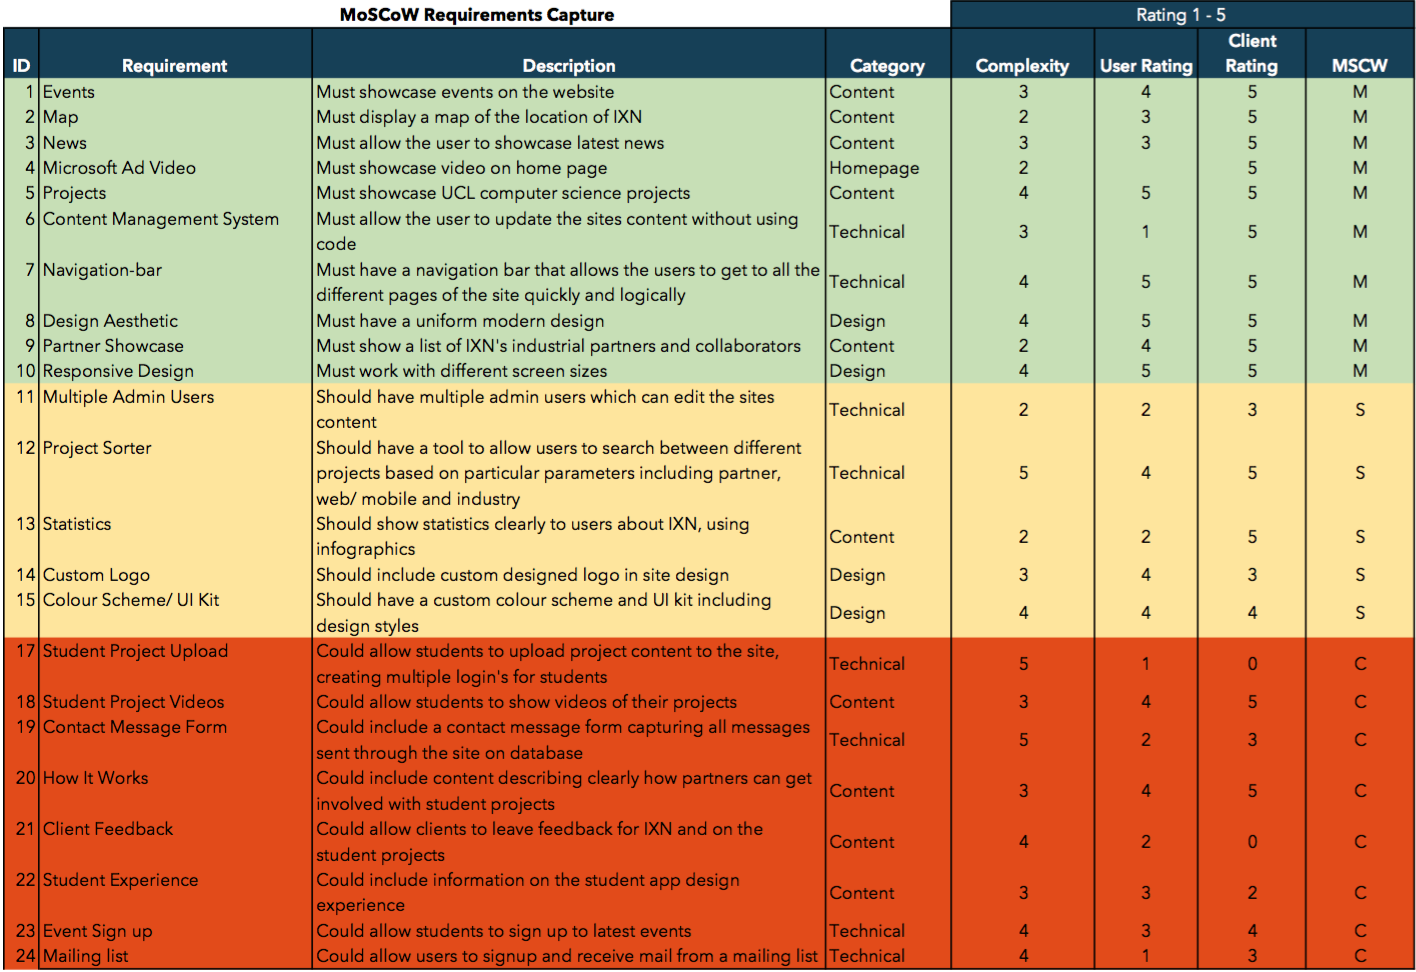
\includegraphics[trim = 0 0 0 0, clip, width=0.7\textwidth]{ph2.png}
      \caption{MoSCoW framework applied to IXN website requirements}
 \end{figure}

\hypertarget{types-of-requirements}{%
\subsection{Types of requirements}\label{types-of-requirements}}

There are two types of requirements web development: functional and
non-functional. The former, are ones which define specific tasks and
activities the project must be able to perform. The latter, are ones
which outline the way a system operates and strongly related to the
architecture of the system \cite{g5}. Due to the nature of a website
used to showcase projects which have already been made, most of the
requirements fall under the functional category, nonetheless, the most
important ones of both types for IXN website are summarized below:

\hypertarget{functional-requirements}{%
\subsubsection{Functional requirements}\label{functional-requirements}}

\begin{itemize}
\tightlist
\item
  Professional and highly polished design suitable for the business
  environment
\item
  Displaying news related and events related to the Industrial Exchange
  network
\item
  Showcasing projects made by the CS department through images and
  videos
\item
  A navigation bar which is always present at the top of the webpage
\item
  Displaying partners of the IXN
\item
  Project Sorting tool
\end{itemize}

\hypertarget{non-functional-requirements}{%
\subsubsection{Non-functional
requirements}\label{non-functional-requirements}}

\begin{itemize}
\tightlist
\item
  Content Management System to be able to update the website without
  having to modify the code directly.
\item
  Scailability when inserting new projects, news and events
\end{itemize}

\hypertarget{technical-research}{%
\section{Technical Research}\label{technical-research}}

\hypertarget{prototyping}{%
\subsection{Prototyping}\label{prototyping}}

Given the importance for the website to display a very accurate,
proficient and effective design a great amount of effort was placed into
prototyping. Various tools were used to turn handmade sketches into a
final prototype. The table below explains which methods have been used
and the reason they have been chosen:

\begin{figure}[H]
      \centering
      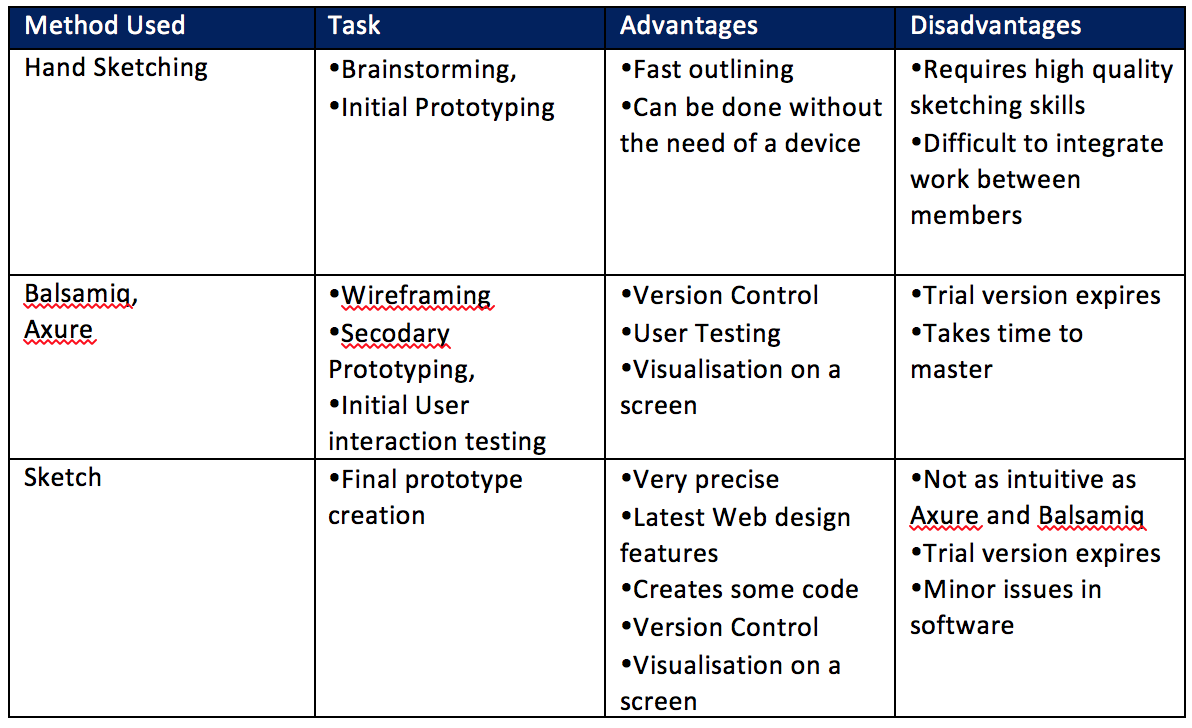
\includegraphics[trim = 0 0 0 0, clip, width=0.7\textwidth]{ph19.png}
      \caption{Prototyping methods and tools used}
 \end{figure}

\hypertarget{content-management-system}{%
\subsection{Content management system}\label{content-management-system}}

A content management system (CMS) is defined as a piece of software that
is designed to provide some level of automation for the tasks required
to effectively manage content. It is usually server-based, interacting
with content stored in a repository, which may be located on the same
server \cite{p1} . In web development, the ultimate purpose of such
tools is to allow an administrative user to edit the content on web page
without having to append HTML directly.

The CMS used for the IXN project was WordPress. There are other free,
open-source CMS options, such as Drupal or Joomla, but WordPress was
selected due to a few critical advantages. These can be boiled down to:
1) Better support options and availability, 2) Superior access to themes
and add-ons and 3) Easy website maintenance.~

\hypertarget{support-options-and-availability}{%
\subsubsection{Support options and
availability~}\label{support-options-and-availability}}

WordPress support is available on a plethora of developer support
channels for web developers and beginners alike on a myriad of
platforms. These include docs, handbooks, codex, Slack channels and
Stack Exchange to name a few. Being the most popular CMS, there are
entire websites dedicated to support in addition to thousands of online
tutorials. Unlike WordPress, finding expert support for Joomla or Drupal
is not quite so simple. All of the platforms provide extensive primary
source documentation, but~because of WordPress's popularity, it
outshines its competitors as far as ease of access to efficient
troubleshooting.~

\hypertarget{access-to-themes-and-add-ons}{%
\subsubsection{Access to themes and
add-ons~}\label{access-to-themes-and-add-ons}}

While Drupal and Joomla also both offer themes and add-ons, the access
and variety are not comparable to WordPress, which offers around 40,000
additional plugins. In Joomla, there is a feature that allows users to
add install from web features for extensions. However, in order to
access a template, a user would still have to manually search templates
and then install them by adding their URL, which is a bit more arduous
that the streamlined WordPress process using the dashboard. Worse still,
Drupal users have to have to exit their site, search for the module and
theme they want, find the zip file URL and submit the URL to the Modules
or Themes page to install them.~

Not only does WordPress take minutes to install, but also the dashboard
interface after the install is simple and easy to navigate. This is
especially useful if you are developing a simple site for a client and
they want to be able to manage and modify the site easily. When
WordPress undergoes updates, the process is seamless and developers
usually won't have to make any changes. It should also be mentioned that
WordPress has an app from which one can manage their site. Joomla's
post-install panel is not as intuitive and has many more features.
Seasoned web developers may~prefer this, but for simplicity, WordPress
wins out. Drupal offers users `distributions', particular to the type of
site that they want to develop. This could be a bit confusing for
beginners. Finally, Drupal's updates can require developer knowledge
\cite{p2} \cite{p3} \cite{p4} .

\hypertarget{bedrock-and-trellis}{%
\subsubsection{Bedrock and Trellis}\label{bedrock-and-trellis}}

Bedrock is a secure way to install and manage WordPress, implementing an
alternative to the conventional WordPress structuring.

Traditionally, WordPress can be installed on both a local device and
also a production server, having a Git repository for a sites theme. In
this case, deployment means a Git pull of the repository from the server
or FTP of the theme. In some cases, the whole site, including WordPress
files can be kept under Git as well \cite{p6} .

This approach is troublesome because when WordPress/plugin updates
occur, the production site can be broken. To illustrate, after writing
code in order update some updated WordPress or plugin functionality, it
is time to deploy. When a developer does so, they must install or update
the correct version of the plugin on the production site, compile
assets, update the theme on the remote server, and then ensure the
plugin has been activated on the production site. This manual and
laborious approach is quite error prone and can lead to downtime.

Bedrock is a modern WordPress stack that brings more automation to web
development and site maintenance and does so using a better folder
structure. (fig 1) It uses PHP doting for environment variables, which
are part of the twelve-factor app, a methodology created by Heroku for
building web apps\cite{p5}. The main goal of this methodology is to
improve work on a growing codebase. The details of underlying principles
of this methodology are beyond the scope of this work, but can be found
in reference 6 \cite{p8} .

\begin{figure}[H]
      \centering
      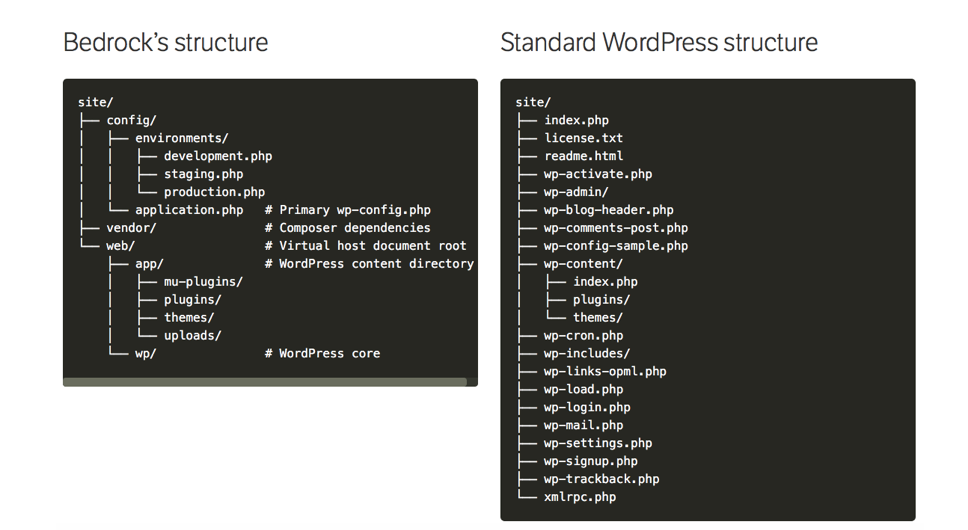
\includegraphics[trim = 0 0 0 0, clip, width=0.7\textwidth]{ph20.png}
      \caption{Difference between Bedrock and standard Wordpress Structure}
 \end{figure}

Composer, a tool for dependency management in PHP, is used to pull in
both dotenv and WordPress, along with WordPress plugins \cite{p7} .
Suppose a developer has a project that depends on a number of libraries
and some of those libraries depend on other libraries. In essence,
Composer allows the developer to declare the libraries they depend on
and finds out the correct versions of packages needed and installs them
into the project \cite{p8} .

Bedrock also makes use of Capistrano, a remote server automation tool,
for automated deployments \cite{p9}. Vagrant is used to implement
easy-to-use development environments. It is a virtual environment
manager with a focus on automation \cite{p10} . Vagrant provides work
environments that are easy to configure, reproducible, and transportable
controlled by a single reliable workflow. To do so, machines are
provisioned on top of a virtualizer, such as VMWare or VirtualBox. Then,
industry-standard provisioning tools such as shell scripts, Chef, or
Puppet, can automatically install and configure software on the virtual
machine \cite{p10} .

The combination of Ansible, an IT automation/server configuration tool,
and bedrock give us Trellis \cite{p11}. Ansible is used for automation
of cloud provisioning, configuration management, application deployment,
and many other IT needs \cite{p12}. The combination of the Bedrock
structure and Ansible automation means that Trellis allows WordPress
developers to create and manage more professional server environments
almost automatically.

An alternative to using Trellis would be MAMP, which has distinct
disadvantages. With MAMP, a developer is tied to the versions of the
software that MAMP precludes. Updates may be made, to PHP 5.6 for
example, but the local MAMP install would be different from your shared
host, or VPS, or dedicated server. The differences between the
environments of your host machine with MAMP and that of a remote server
can cause issues during deployment. This can also cause problems when
something goes wrong on your production server and you can't replicate
it on your local machine or vice versa \cite{p13} . Trellis creates
staging and production environments, meaning that's the
staging/production server matches your development virtual machine.

\hypertarget{front-end}{%
\subsection{Front-End}\label{front-end}}

As the name would suggest, front-end development encompasses the
creation of the parts of a website with which the user interacts,
through the use of technologies such as HTML, CSS, and JavaScript. In
other words, this is where the site's content, styling and dynamic
interface is coded.

HyperText Markup Language, or HTML, is the backbone of the IXN website.
This is where the site's content is kept. It is in the HTML documents
where a developer uses PHP to connect the site with the content
management system.

The site's styling was done using SCSS, a version of cascading style
sheet (CSS) written for SASS, a program written in Ruby that assembles
CSS style sheets for a browser. The advantage of using SASS is that is
has added functionality, allowing the use of variables, nested rules,
mixins and more within CSS-compatible syntax \cite{p14} .

Because the IXN website will be accessed from many different devices
with different screen sizes, responsive design principle were used
during front end development. In order to achieve a consistent,
responsive interface, Bootstrap 4, a front-end web framework based on
CSS styling, was used. It has set of fixed classes that allow developers
to quickly create applications that scale to devices of all sizes.
Additionally, Bootstrap aids developers in adding common components such
as navigation bars and panels to a site. It has become the industry
standard for responsive web development \cite{p15} .

In order to add dynamic functionality to the IXN website JavaScript (JS)
was used. JS is a front-end development language which many websites
employ and it is supported by all modern web browsers. JQuery is a
JavaScript library that simplifies animation, event handling and much
more. It was also used to add functionality to the IXN website
\cite{p16}.

\begin{figure}[H]
      \centering
      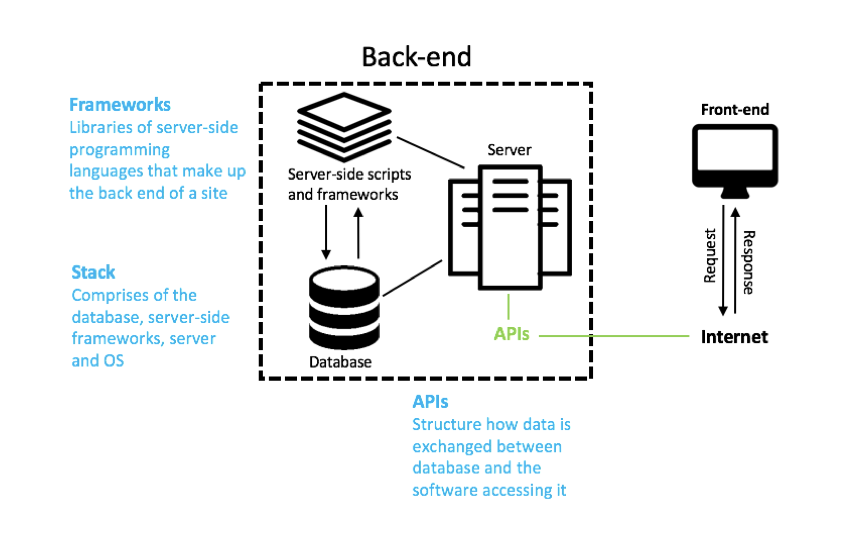
\includegraphics[trim = 0 0 0 0, clip, width=0.7\textwidth]{ph18.png}
      \caption{Front-End and Back-End interaction}
 \end{figure}

\hypertarget{back-end}{%
\subsection{Back-End}\label{back-end}}

Back end development refers to the server -side code written to ensure
that a site is robust and usable. This is the code that is run on the
server and is responsible for things such as database interactions,
logic, and calculations. For the IXN website, PHP was used for
server-side scripting in order to query the MariaDB database \cite{p17}
.

Since WordPress was used as the content management system, it was also
deployed on our server so that content could be updated via the
user-friendly dashboard. This would then update the database, and
strategically placed PHP embedded in HTML would then be used to display
the content on the appropriate part of the site.

Blade, a templating engine was used in conjunction with PHP, which can
be detected when the file extension blade.php is used. Blade employs the
concepts of template inheritance and sections. The @section notation
allows for easy organization of a site and it can be see embedded in the
html. The @extends notation can be used in order to inherit other
layouts. These tools are extremely convenient for effectively organizing
code \cite{p18} .

\begin{figure}[H]
      \centering
      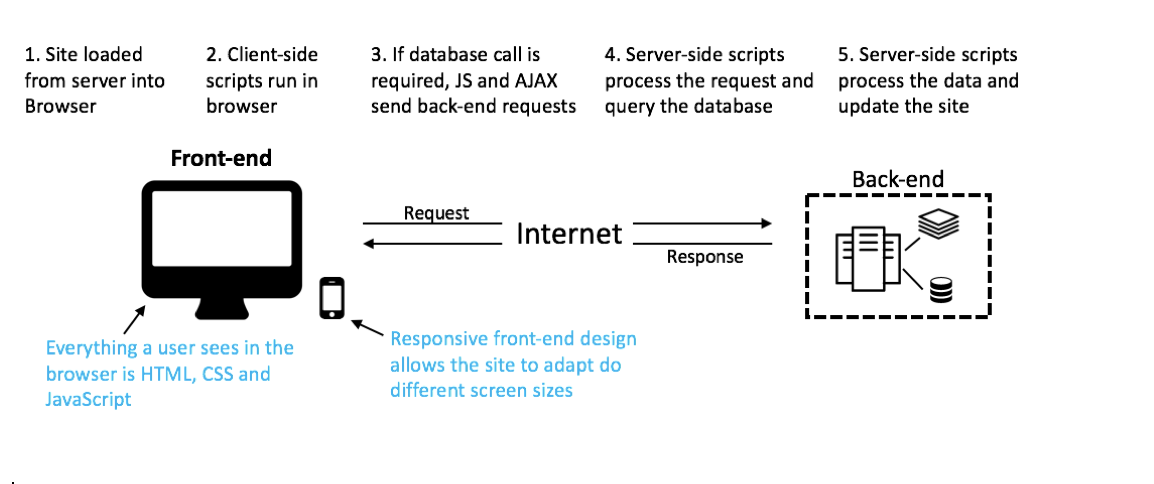
\includegraphics[trim = 0 0 0 0, clip, width=0.7\textwidth]{ph17.png}
      \caption{Front-End and Back-End interaction}
 \end{figure}

\hypertarget{system-architecture}{%
\section{System Architecture}\label{system-architecture}}

In order to be able to create a high performance website, using the
latest technologies to optimises run time and speed up the design
process; a stack of Wordpress technologies were used in three tier
system architecture. The stack was run across both local and production
servers enabling a testing environment which was fully representative of
the production server while all code could be kept offline.

The full open source Roots stack \cite{rootsweb} was selected as it
provided all the tools and structure required to develop the project to
a professional standard. Figure \ref{systemarchitecture} shows the
relationship between the three roots technologies; Sage, Bedrock and
Trellis, and their relationship to the system architecture.

\begin{figure}[H]
\centering
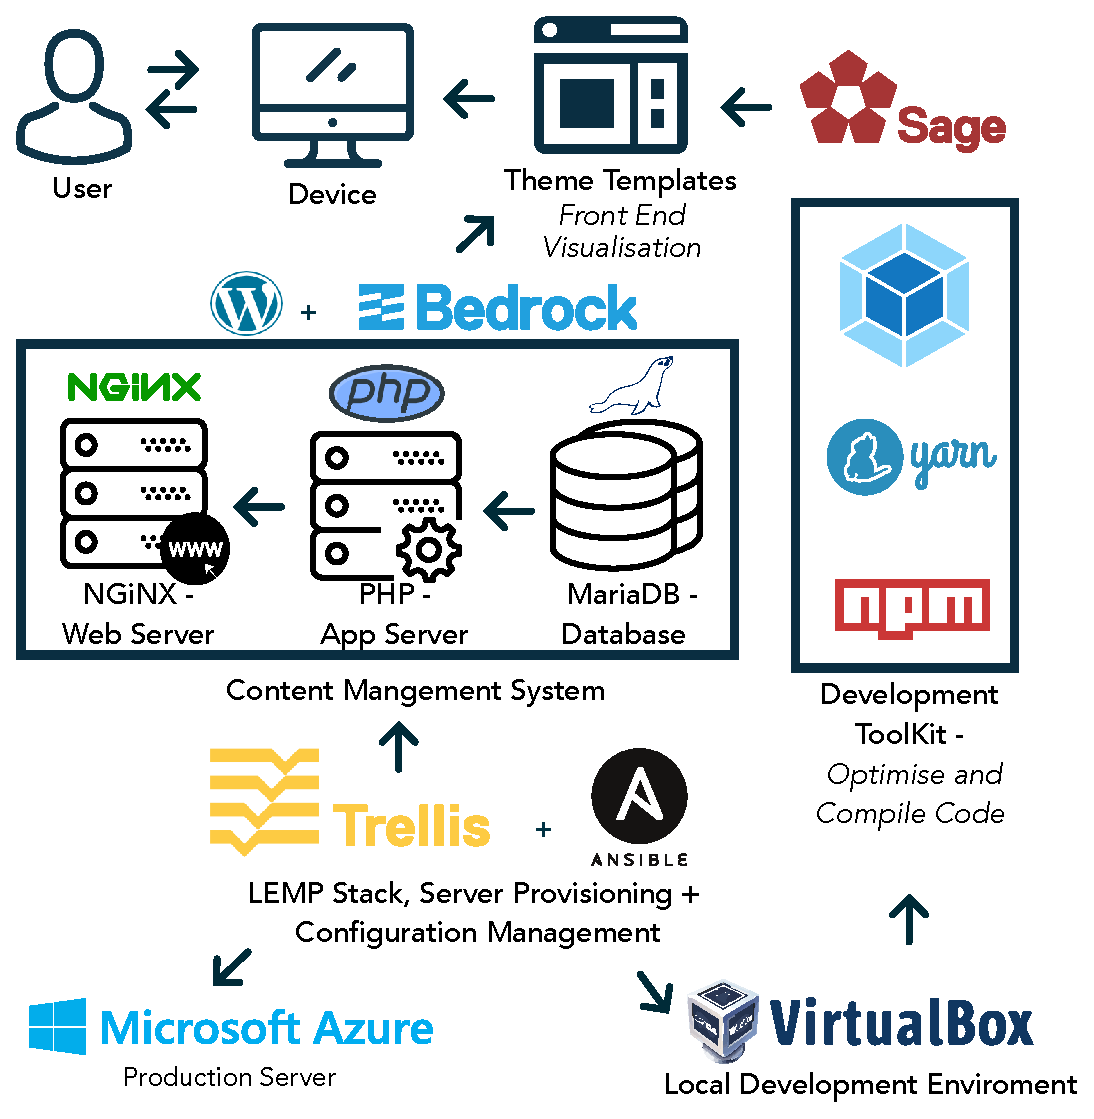
\includegraphics[trim = 0 0 0 0, clip, width=0.85\textwidth]{SystemArchitecture.eps}
\caption{Diagram showing the websites systems architecture, highlighting the relationship between different technologies}
\label{systemarchitecture}
\end{figure}

\newpage

\hypertarget{design-principles}{%
\section{Design Principles}\label{design-principles}}

\hypertarget{implementation}{%
\section{Implementation}\label{implementation}}

\hypertarget{development-tools}{%
\subsection{Development Tools}\label{development-tools}}

After prototyping using Sketch was completed, each team member took
responsibility for the development of specific sections of the site.
CodePen was used to make each component for the website before all of
the sections were integrated into the appropriate page layouts. The
benefit of using CodePen is that HTML, CSS and JavaScript code can be
written in the browser, and compiled in real time, with the result
visible in the same window. \cite{p19} Ultimately, it allows for faster
development and easy troubleshooting.

From CodePen, the front-end code was integrated into the site's pages
using text editors such as Atom and Sublime, each member had their own
preferences. This was where PHP was added. In the later stages of
development, all of the code was edited and written using text editors.

\#\#Code Organization

\hypertarget{remote-server}{%
\subsubsection{Remote Server}\label{remote-server}}

Trellis was used to set up a remote server to be used for the IXN
website's development. When Trellis sets up a local development
environment, it automatically creates a server, provisions it, and
installs WordPress \cite{p21} . This is done by Vagrant in Trellis, by
which a Vagrantfile uses the Ansible provisioner to run dev.yml to set
up a virtual machine on the WordPress site using VirtualBox \cite{p22} .

This was done through a few simple steps. First the site was configured
based on the WordPress Sites docs. Then,
group\_vars/development/wordpress\_sites.yml and
group\_vars/development/vault.yml were edited. Finally, vagrant up was
run from the command line from the Trellis folder in the site directory.

To create a remote server from the remote development environment, a
couple of extra steps were needed: Provision and Deploy. Provisioning
was done in order to ensure MariaDB and Nginx were installed, Nginx was
configured, and a database was set up for the IXN site. The server was
provisioned using server.yml. Deployment was done using deploy.yml which
took the codebase from GitHub, ran Composer, created config files and
reloaded Nginx. \cite{p23}.

\hypertarget{github}{%
\subsubsection{GitHub}\label{github}}

Finally, GitHub was used for collaboration. Git is a version control
system, allowing revisions in the code to be stored neatly and
chronologically. The changes can then be seen by other developers who
can download and modify it. \cite{p20} GitHub is the community of
developers and where they store their work.

For the IXN website there was a group repository where code was shared
and updated. In order to organize to code and ensure the integrity of
the site, five branches were made. There was a branch made for each
individual member (Alexcode, PhoebeCode and GioCode). This is where code
was written the majority of the time. When updates were finalized, code
from these branches was then pushed to the Dev branch. After this code
was reviewed and if there were no clashes, the code was then pushed to
the master branch which housed the cleanest and most current version of
the site at any given time.

\begin{figure}[H]
      \centering
      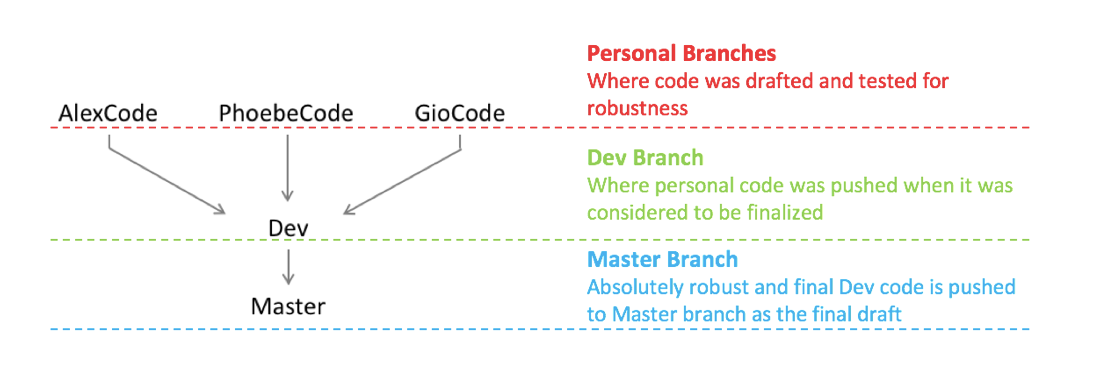
\includegraphics[trim = 0 0 0 0, clip, width=0.7\textwidth]{ph15.png}
      \caption{Post implementation annotated MoSCoW}
 \end{figure}

\# Site Map \& Page Flow

\begin{figure}[H]
      \centering
      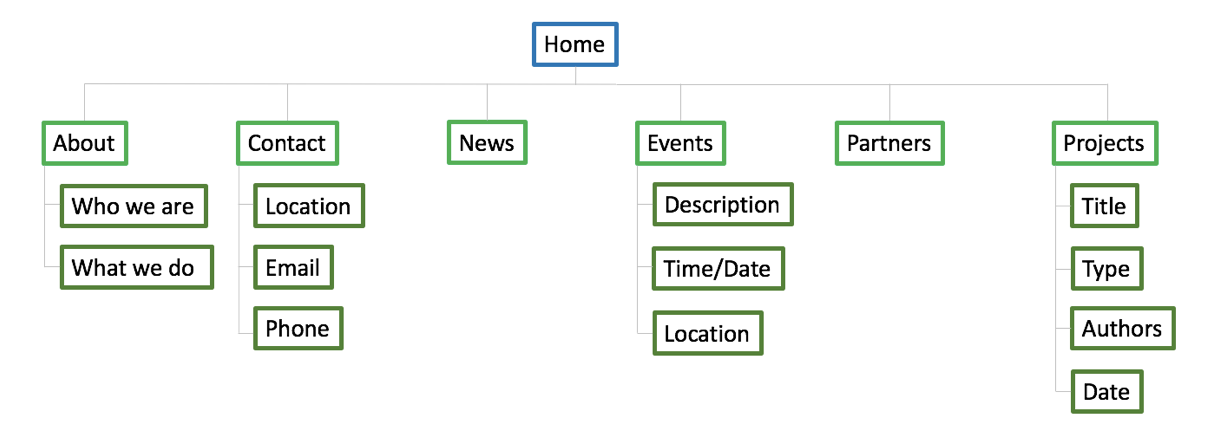
\includegraphics[trim = 0 0 0 0, clip, width=0.7\textwidth]{ph16.png}
      \caption{Site Map}
 \end{figure}

\hypertarget{testing}{%
\section{Testing}\label{testing}}

\hypertarget{compatibility-responsiveness}{%
\subsection{Compatibility \&
Responsiveness}\label{compatibility-responsiveness}}

The team underwent research on which browser simulators to use while for
testing compatibility and responsiveness of the IXN website.
BrowserStack because of its free trial plan and the span of emulators
was the tool chosen to perform the tests \cite{g6}. BrowserStack, in
fact, offered the possibility of testing the IXN website on a multitude
of Operating System, Devices and Browsers. Moreover, to integrate and
broaden the results of the tests the team tested the IXN project on
physical devices as well. The results obtained for desktops and laptops
are displayed below:

\begin{figure}[H]
      \centering
      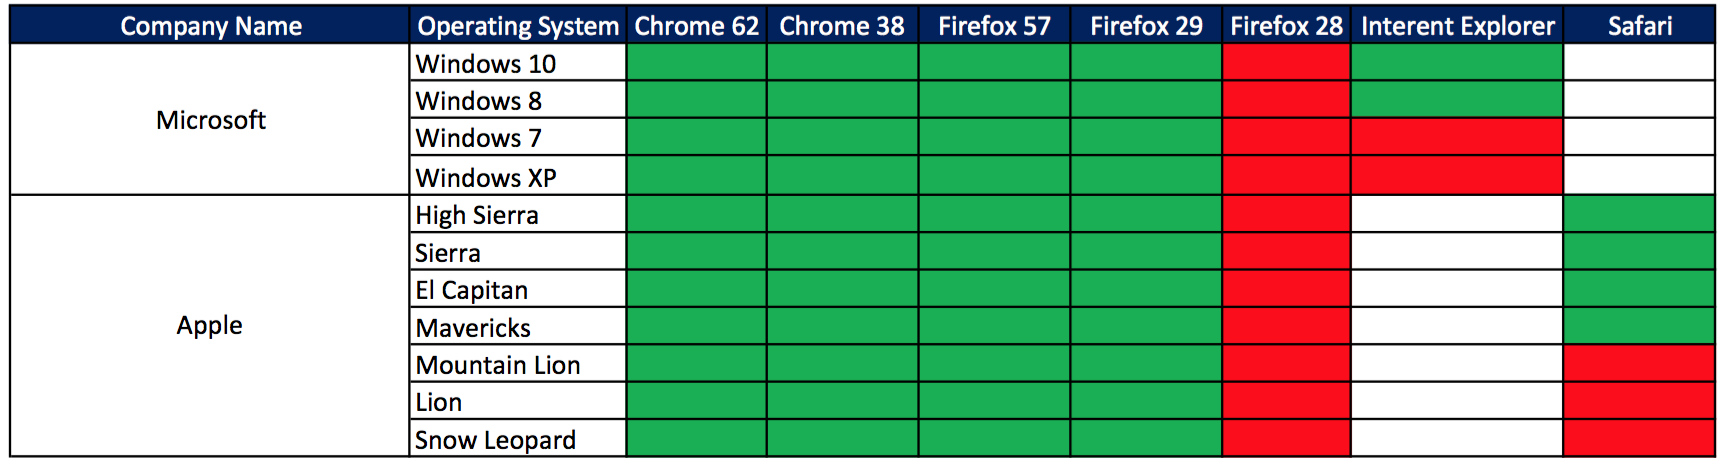
\includegraphics[trim = 0 0 0 0, clip, width=0.7\textwidth]{ph7.png}
      \caption{Laptop/Desktop browser testing results}
 \end{figure}

As regards testing on mobile devices BrowserStack was the platform
chosen. Moreover, as not all of the emulators were available on free
trial, physical device testing also played a very important part. The
webpage appears fully responsive on modern software versions, however,
as occurred with the desktop devices older versions of software (around
2012/2013) struggle with the desing, SCSS and Bootstrap 4. The mobile
testing results are displayed below:

\begin{figure}[H]
      \centering
      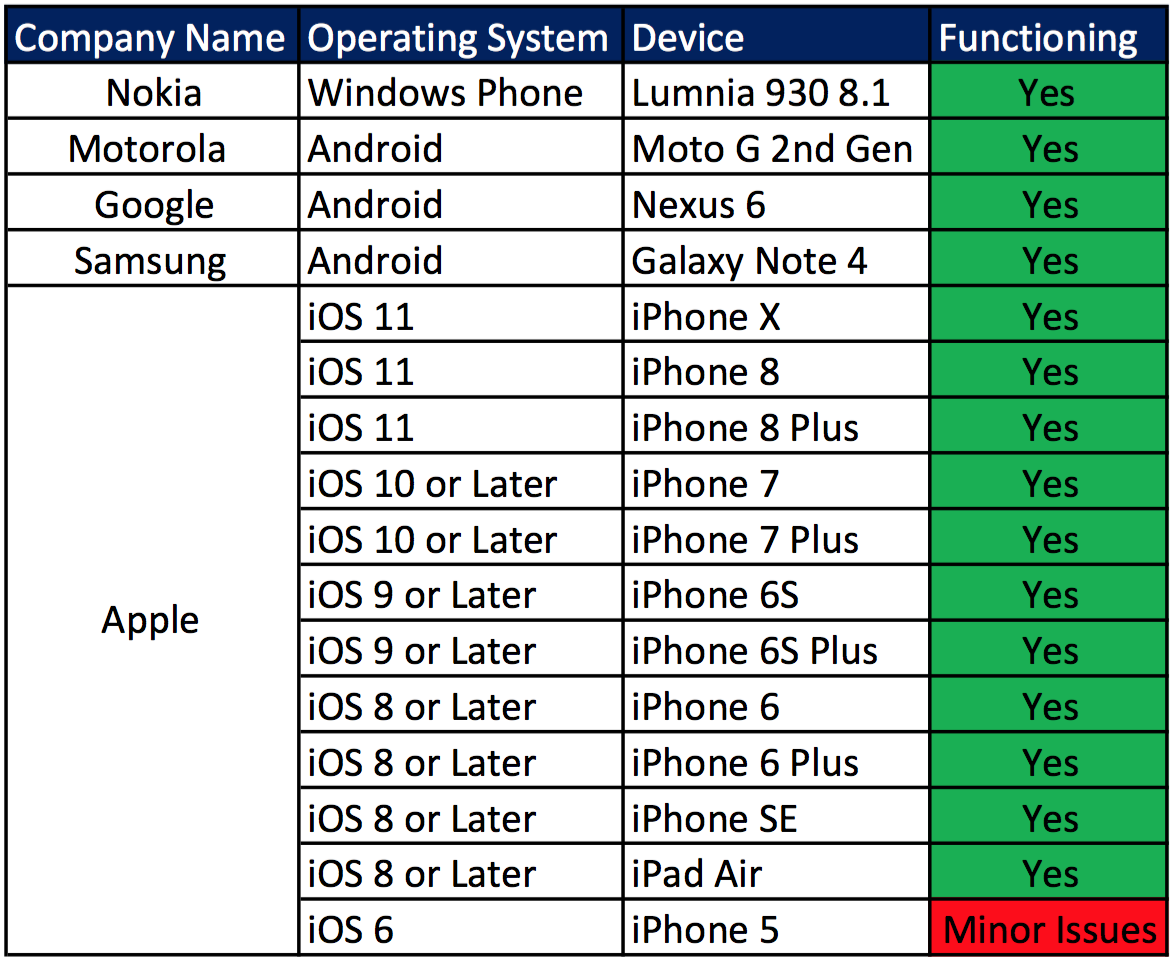
\includegraphics[trim = 0 0 0 0, clip, width=0.7\textwidth]{ph8.png}
      \caption{Laptop/Desktop browser testing results}
 \end{figure}

\hypertarget{server-stability-issues}{%
\subsection{Server Stability Issues}\label{server-stability-issues}}

The team has encountered issues in launching the website trough
Microsoft Azure. The website sporadically shows that the page is not
redirecting properly or that the page is in a redirect loop. The problem
seems to disappear after the page is reloaded a second time. The team
was not able to fix this matter. Future teams working in the IXN project
will have to improve the relationship between the website and the Azure
servers to increase stability and avoid the occasional redirect errors.

\hypertarget{acceptance-testing}{%
\subsection{Acceptance Testing}\label{acceptance-testing}}

The IXN User Acceptance Testing (UAT) has been generated around the
requirements of the website \cite{g7} . In fact, Use Cases have been
used to pick and prepare tasks for users to perform while testing. The
procedure the IXN team has followed for User Acceptance Testing is the
following: 1. Design tests for users to cover functional scenarios of
the website 2. Select a varied background testing team, in accordance to
the main users of the website 3. Perform the tests and record the
results 4. Bug fix with the faults encountered, or improve the defective
features features

For the IXN website UAT 35 individuals of varied technological knowledge
were asked to complete the tasks given and the time of completion was
recorded. The table below summarizes the results obtained:

\begin{figure}[H]
      \centering
      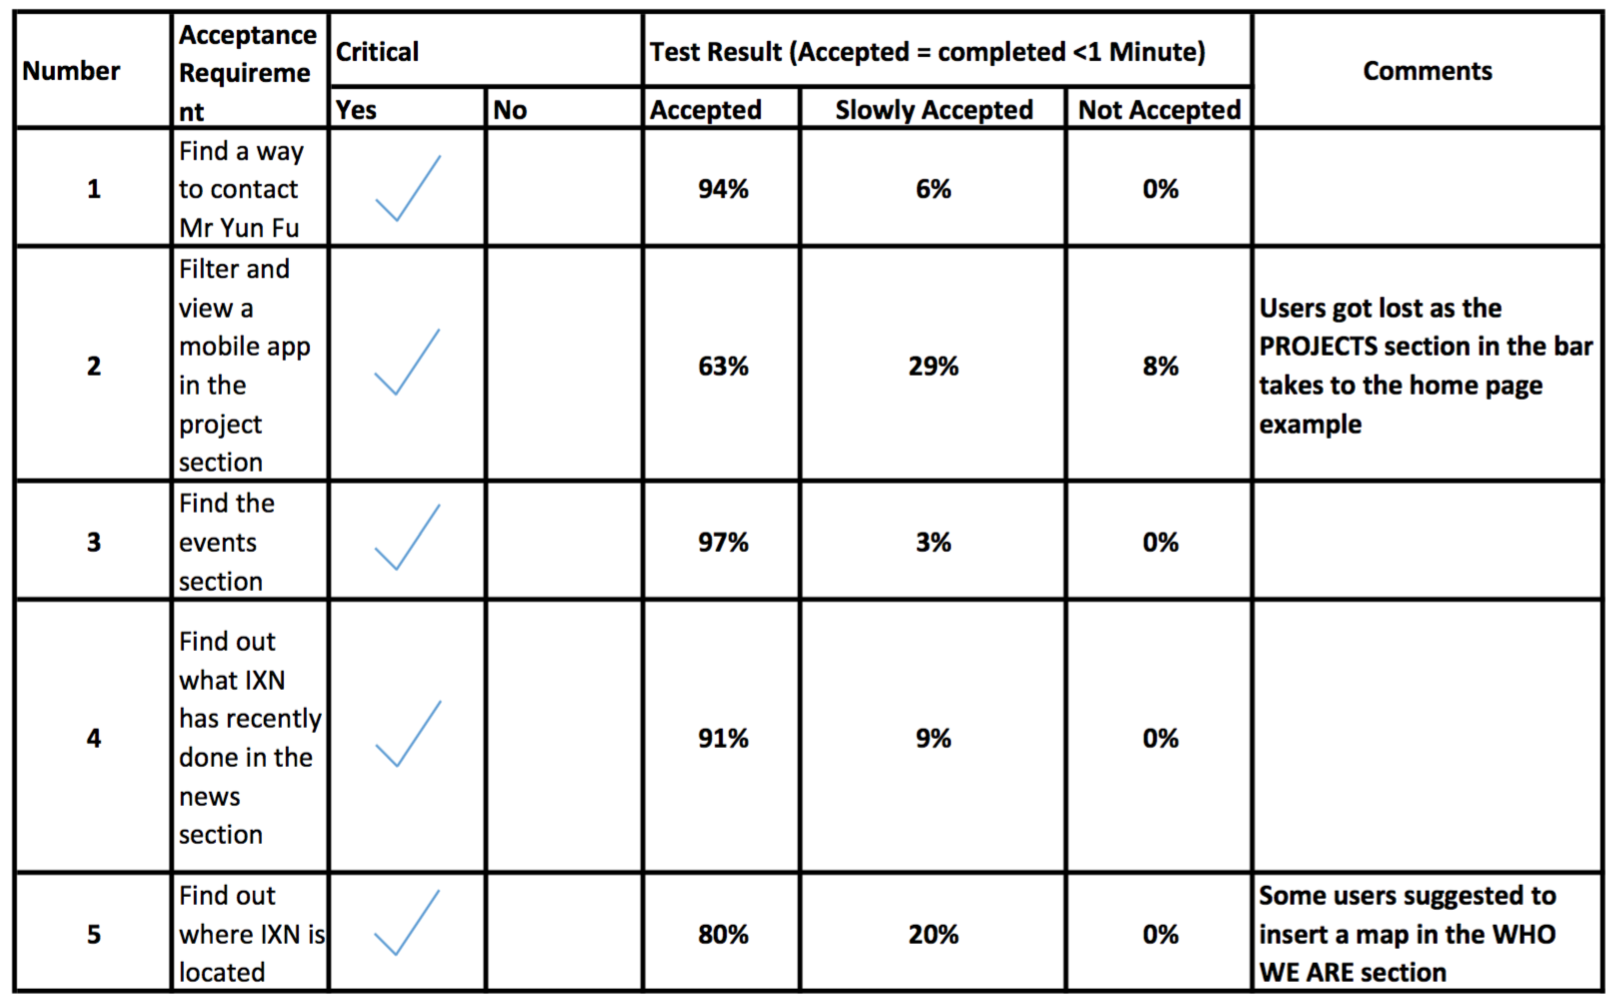
\includegraphics[trim = 0 0 0 0, clip, width=0.7\textwidth]{ph4.png}
      \caption{User Acceptance Testing summarized results}
 \end{figure}

\hypertarget{error-guessing}{%
\subsection{Error Guessing}\label{error-guessing}}

Error guessing has been put into practice by making the most of the
expertise of fellow UCL Computer Science Students. The IXN team asked
members of the department of Computer Science to come up with, consider
and assess circumstances in which the software behind the website might
have had problems in coping with the requests made. The efficiency of
this testing technique depends on the tester's abilities. In the case of
the IXN website some minor bugs were spotted in the news section.
Consequently, the team went on to fixing them.

\hypertarget{conclusion}{%
\section{Conclusion}\label{conclusion}}

\hypertarget{requirements-accomplishments}{%
\subsection{Requirements
Accomplishments}\label{requirements-accomplishments}}

Comparing the initial MoSCoW to the achievements obtained by the team it
is visible that all of the ``Must'' (in green) and ``Should'' (in
yellow)have requirements have been fulfilled. An extra ``Could'' (in
red) feature has been included to give a more comprehensive user
experience. An annotated MoSCoW, explaining how the requirements have
been implemented, can be found below:

\begin{figure}[H]
      \centering
      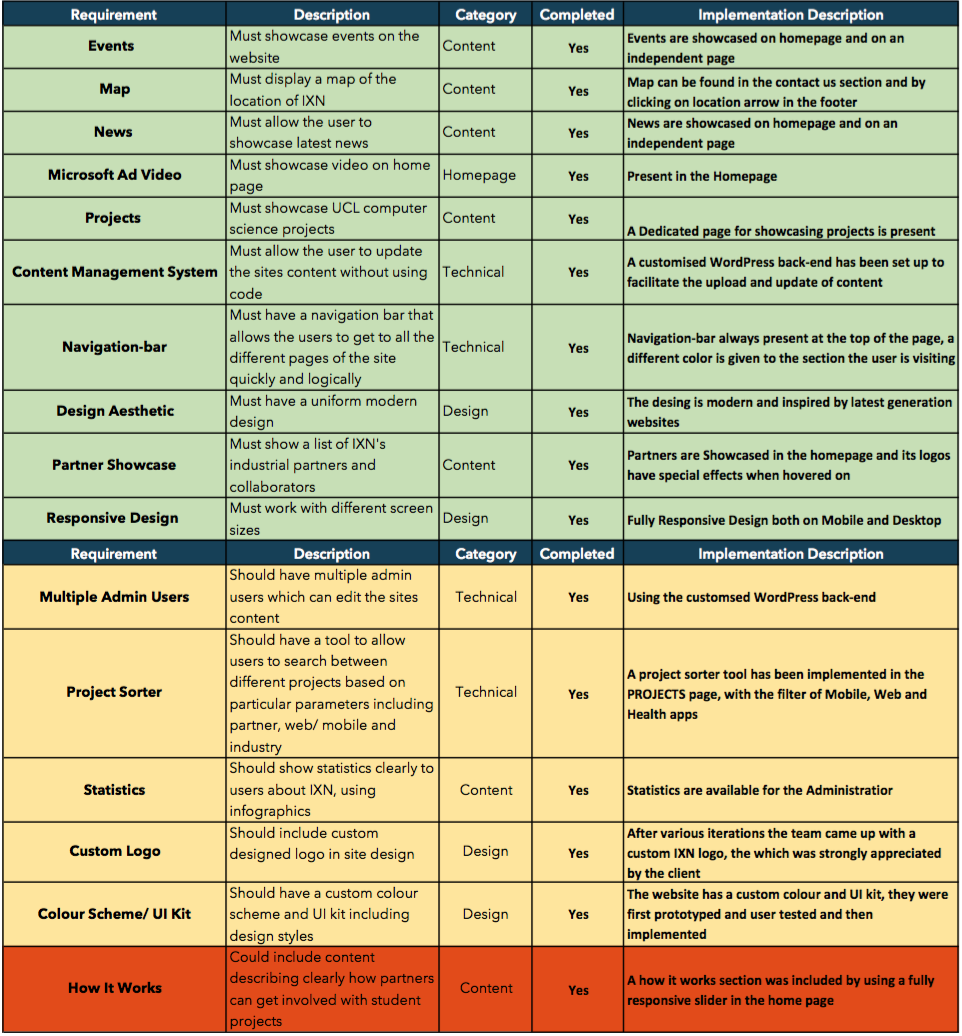
\includegraphics[trim = 0 0 0 0, clip, width=0.7\textwidth]{ph5.png}
      \caption{Post implementation annotated MoSCoW}
 \end{figure}

\hypertarget{team-achievements}{%
\subsection{Team achievements}\label{team-achievements}}

Teamwork always has its advantages and disadvantages. The IXN team had
to face some issues related to the background knowledge, the workload
division and the different culture of its team members. There have been
times of disagreement between team members, however, through open minded
discussion, honesty and respect every individual gained experience and
skills from the creation of the website and cooperating with other
people.

The team was happy with the results obtained with the website, some
gains in the quality of the website could have been obtained by having
access to some costly design, implementation and testing tools. However,
the team was proud of demonstrating that, even with a very limited
budget, effort and determination can make up for not having full access
to all the latest tools and platforms.

\hypertarget{critical-evaluation-future-development}{%
\subsection{Critical Evaluation \& Future
Development}\label{critical-evaluation-future-development}}

The project was highly design focused. Therefore, the team tried hard to
make it attractive, simple to use and professional with the latest tools
and devices available at this day and age. However, in a few years' time
even all the effort put in by the team will result outdated, obsolete
and the website would loose its efficacy \cite{g8} . The role of the
next teams working on the IXN website will, therefore, be to build upon
the foundations that have been created by updating and continuously
rejuvenating the website. A task besides the design features of the
website that future teams will have to take into account is to improve
Azure server stability, to avoid occasional redirect errors that the
website is currently facing. Moreover, the additional and less requested
requirements of the ``Could'' section of the MoSCoW can be taken
consideration and implemented. A commented version of the ``Could''
portion, explaining how the features can be realized, is present below:

\begin{figure}[H]
      \centering
      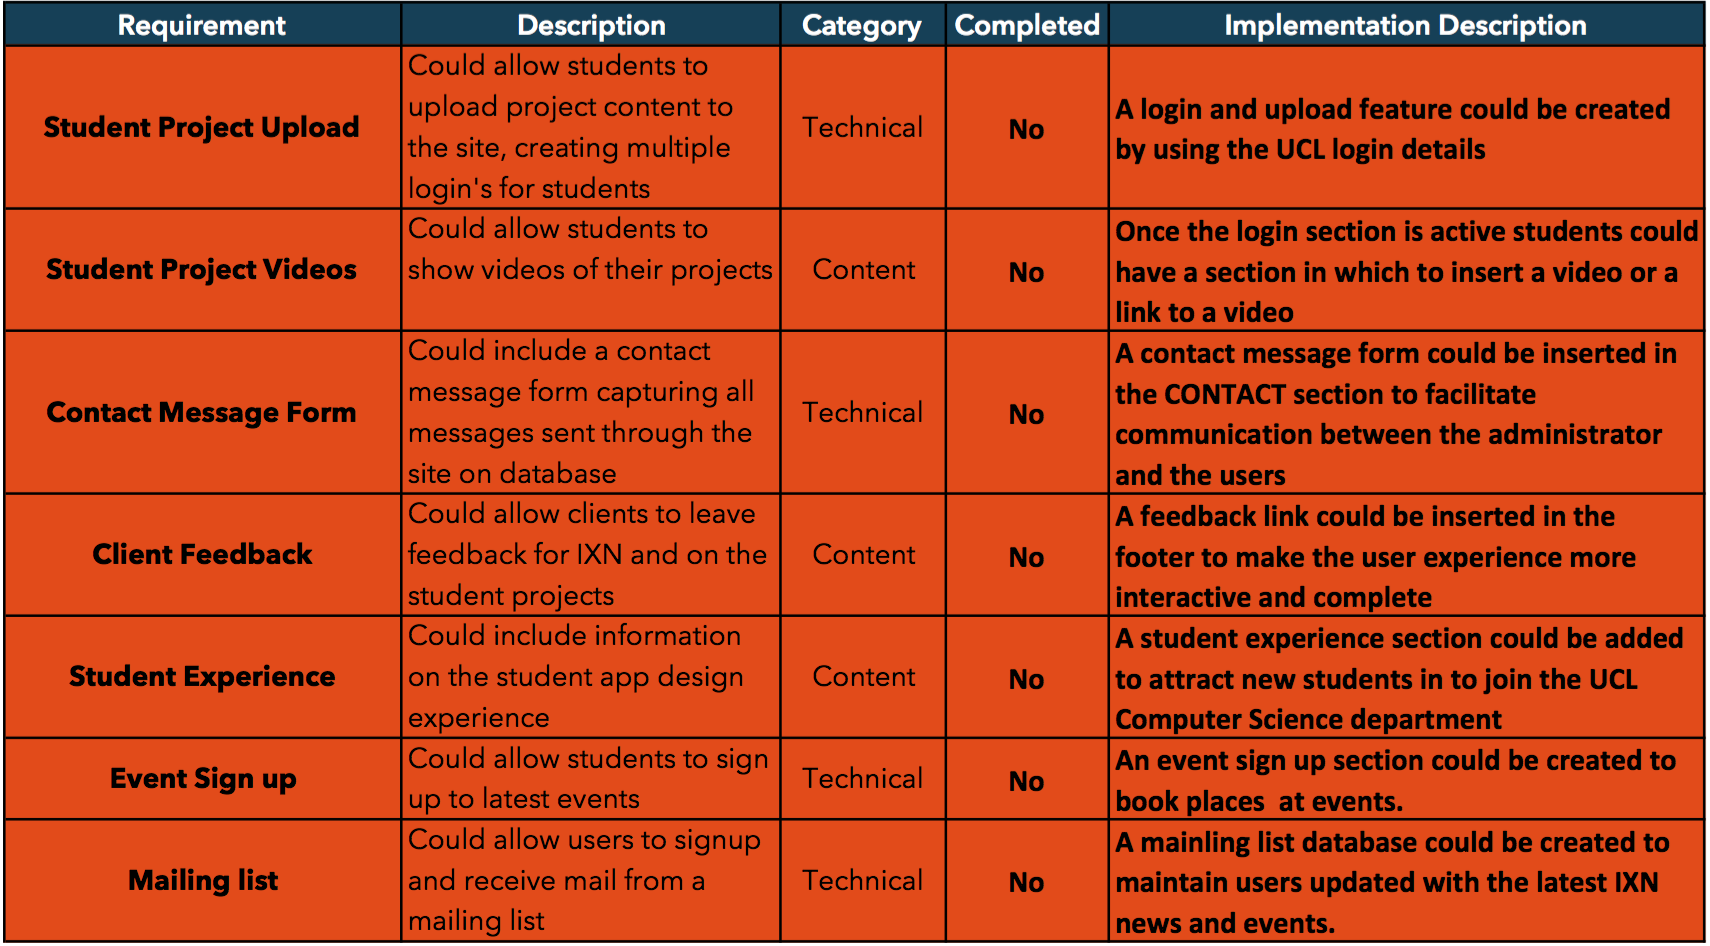
\includegraphics[trim = 0 0 0 0, clip, width=0.7\textwidth]{ph6.png}
      \caption{Possible features to be implemented in the future}
 \end{figure}
